\chapter{Deep Neural Network Compression}\label{chap:sota}

\localtableofcontents

\section{Introduction}\label{sec:sota:intro}

% region: intro
The fast development of neural networks has led, on the one hand, to the
enhancement of their performance, but also, on the other hand, to a significant
growth in size and parameter count. The rapid evolution and adoption of these
networks has given rise to various applications
\cite{DBLP:conf/nips/KrizhevskySH12,DBLP:conf/emnlp/BudzianowskiV19,silver2018general,jumper2021highly},
particularly embedded ones\cite{kim2020review,kuutti2020survey}, whose resources
are highly constrained in terms of computing power, energy consumption and
memory footprint. Alongside the increase in the size of these networks,
compression techniques
\cite{DBLP:conf/nips/CunDS89,DBLP:journals/corr/HanMD15,DBLP:conf/nips/HanPTD15}
have been devised, in order to enable the use of these algorithms in embedded
applications or resource-constrained environments.\\

This chapter focuses on state-of-the-art neural network compression methods,
predominantly based on various operations applied to the weights of an already
existing large neural network. This chapter is organised as follows:
\Cref{sec:sota:fast_convolutions} examines fast convolution techniques, which
aim to accelerate the computation of convolutions in neural networks, thereby
reducing both the runtime and computational resources required. Thereafter,
\cref{sec:sota:teaching_paradigm} delves into \ac{KD}, a process by which the
knowledge of a larger, more complex network (referred to as the \emph{teacher})
is transferred to a smaller and more efficient network (called the
\emph{student}), enabling the latter to achieve comparable performance with a
reduced footprint. Subsequently, \cref{sec:sota:archi_design} explores
architecture design methods that aim at producing more efficient and effective
networks. \Cref{sec:sota:efficient_archi} details ad-hoc architectures, referred
to as \emph{Efficient Architectures}. These architectures are lightweight
networks that revolve around a core technique to reduce their size while
preserving performance as much as possible. Hence, \cref{sec:sota:nas} discusses
\ac{NAS}, a method that automates the discovery of optimal network architectures
tailored to specific tasks or constraints, potentially leading to more compact
and efficient designs. Afterwards, \cref{sec:sota:refining_existing} presents
two categories of techniques that harness an existing neural network and refine
its architecture to produce a more compact and efficient model. First,
\cref{sec:sota:quantisation} focuses on \emph{quantisation} and
\emph{binarisation} techniques, which aim to lower the numerical precision of
weights and activations of networks in order to speed up their computation and
reduce their memory footprint. Lastly, \cref{sec:sota:pruning} considers neural
network pruning, which seeks to remove redundant or insignificant connections and
weights from networks, resulting in sparser and more computationally efficient
models.\\

%TODO: faire une mindmap des méthodes

% endregion: intro

\section{Accelerating Computations in Neural Networks}\label{sec:sota:fast_convolutions}

Among various operations and functions used in neural networks, two fundamental
mathematical operations, convolution and matrix multiplication are used
extensively and are the backbone of most computations in neural networks.
However, performing these operations can be computationally demanding,
particularly with large and complex networks. This may lead to long computation
times, posing a challenge for real-time or resource-limited applications. To
mitigate this issue, some research efforts have focused on developing techniques
to speed up these operations. These strategies encompass optimizing the
underlying algorithms to leveraging hardware acceleration, with the objective of
enhancing the speed and efficiency of neural network computations.\\


\subsection{\acl{FFT}}\label{sec:sota:fft}
The most popular algorithms for
accelerating convolution operations rely on the \ac{FFT}
\cite{DBLP:conf/nips/ChiJM20,DBLP:journals/npl/LinY19,DBLP:conf/pkdd/PrattWCZ17},
and leverage the Convolution Theorem. The Convolution Theorem states that the
convolution of two signals in the source domain is the product of the two
signals in the Fourier domain, as shown in \cref{eqn:sota:conv_theorem_fourier}:\\

\begin{equation}
  \label{eqn:sota:conv_theorem_fourier}
  F(x * y) = F(x) \cdot F(y)
\end{equation}\\

\noindent where $x$ and $y$ are the two signals in the source domain, $x*y$ is
the convolution of $x$ and $y$ and finally $F(x)$ and $F(y)$ are the Fourier
transforms of $x$ and $y$, respectively. Then, to obtain the result of the
convolution in the source domain, the inverse Fourier transform, denoted
$F^{-1}$, is applied as follows:\\

\begin{equation}
  x * y = F^{-1}(F(x) \cdot F(y))
\end{equation}\\

\noindent The convolution theorem allows for faster computation of the 2D
convolution by using the \ac{FFT} to compute the convolution in the frequency
domain, and the inverse \ac{FFT} to convert the result back to the source domain
\cite{oppenheim1997signals}.

\subsection{Optimised Matrix Multiplication Algorithms}\label{sec:sota:matrix_multiplication}

It is possible to accelerate matrix multiplication by directly optimising the
underlying algorithm. The  Strassen algorithm \cite{strassen1969gaussian}, used
in \cite{DBLP:conf/icann/CongX14}, is a fast method for matrix multiplication
that reduces the computational complexity from the standard $\mathcal{O}(n^{3})$
to approximately $\mathcal{O}(n^{2.807})$ by recursively dividing the matrices
of size $n$ into 4 submatrices of size $\frac{n}{2} \times \frac{n}{2}$,
reorganising and combining these multiplications to perform only 7 instead of 8
matrix multiplications (see
\cref{eqn:sota:matrix_multiplication_strassen,eqn:sota:matrix_multiplication_strassen_result}).\\

Considering a matrix multiplication of two square matrices $A$ and $B$ of size
$2n$ with $n\in\mathbb{N}$, defined in \cref{eqn:sota:matrix_multiplication},
the output of the standard bloc matrix multiplication, referred to as $C$, is
defined in \cref{eqn:sota:matrix_multiplication_result}. Note that $A_{ij}$ and
$B_{ij}$ are either a scalar if $n=1$, or a matrix of size $\frac{n}{2} \times
\frac{n}{2}$.\\

\begin{equation}
  \label{eqn:sota:matrix_multiplication}
  A = \begin{bmatrix} A_{11} & A_{12} \\ A_{21} & A_{22} \end{bmatrix},
  B = \begin{bmatrix} B_{11} & B_{12} \\ B_{21} & B_{22} \end{bmatrix}
\end{equation}\\

\noindent The computation of $C$ requires 8 matrix multiplications, as shown in
\cref{eqn:sota:matrix_multiplication_result}.\\
\begin{equation}
  \label{eqn:sota:matrix_multiplication_result}
  C = A \cdot B = \begin{bmatrix} A_{11}B_{11} + A_{12}B_{21} & A_{11}B_{12} + A_{12}B_{22} \\ A_{21}B_{11} + A_{22}B_{21} & A_{21}B_{12} + A_{22}B_{22} \end{bmatrix}
\end{equation}\\

\noindent The Strassen algorithm reduces the number of multiplications to 7 by
defining the following 7 products, referred to as $P_{i}$, with $i\in \llbracket
1;7 \rrbracket$:\\

\begin{equation}
  \label{eqn:sota:matrix_multiplication_strassen}
  \begin{aligned}
    P_{1} & = (A_{11} + A_{22})(B_{11} + B_{22}) \\
    P_{2} & = (A_{21} + A_{22})B_{11}            \\
    P_{3} & = A_{11}(B_{12} - B_{22})            \\
    P_{4} & = A_{22}(B_{21} - B_{11})            \\
    P_{5} & = (A_{11} + A_{12})B_{22}            \\
    P_{6} & = (A_{21} - A_{11})(B_{11} + B_{12}) \\
    P_{7} & = (A_{12} - A_{22})(B_{21} + B_{22})
  \end{aligned}
\end{equation}\\

\noindent The result of the matrix multiplication is then obtained by combining
these products, as shown in
\cref{eqn:sota:matrix_multiplication_strassen_result}.\\

\begin{equation}
  \label{eqn:sota:matrix_multiplication_strassen_result}
  C = \begin{bmatrix}
    P_{1} + P_{4} - P_{5} + P_{7} & P_{3} + P_{5}                 \\
    P_{2} + P_{4}                 & P_{1} - P_{2} + P_{3} + P_{6}
  \end{bmatrix}
\end{equation}\\

\noindent The Strassen algorithm has later been refined by
\citeauthor{coppersmith1987matrix}, who introduced the Coppersmith-Winograd
algorithm \cite{coppersmith1987matrix}. The latter brings down the complexity to
$\mathcal{O}(n^{2.376})$. This algorithm is used in various works, mostly
targeted towards a specific \ac{FPGA} processor
\cite{liu2018efficient,lu2018spwa,wang2020winonn}.\\

\subsection{Leveraging Matrix Structures}\label{sec:sota:matrix_structures}
Using a particular matrix structure also speeds up the standard operations used
in a neural network. Fully connected layers can be effectively accelerated by
forcing the use of specific matrix structures. For instance,
\citeauthor{DBLP:conf/iccv/ChengYFKCC15} devised a method where dense layers
standard operation is replaced by a circulant projection
\cite{DBLP:conf/iccv/ChengYFKCC15}. The circulant matrix can be stored in a
memory-efficient way and can be further sped up with \ac{FFT}. $C$ is an example
of a circulant matrix (see \cref{eqn:sota:circulant_matrix}).\\

\begin{equation}
  \label{eqn:sota:circulant_matrix}
  C =
  \begin{pmatrix}
    a & b & c & d \\
    d & a & b & c \\
    c & d & a & b \\
    b & c & d & a
  \end{pmatrix}
  \quad
  T =
  \begin{pmatrix}
    a & b & c & d \\
    e & a & b & c \\
    f & e & a & b \\
    g & f & e & a \\
  \end{pmatrix}
\end{equation}\\

Likewise, convolutional operations can be accelerated thanks to Toeplitz
matrices. A Toeplitz matrix, or diagonal-constant matrix, has the unique
characteristic of each descending diagonal from left to right being constant.
$T$ is an example of a Toeplitz matrix (see \cref{eqn:sota:circulant_matrix}).
This property is particularly useful for convolutions, as they can be expressed
as a multiplication by a Toeplitz matrix \cite{gray2006toeplitz}, as shown in
\cref{eqn:sota:toeplitz_matrix_conv}. This algorithm has been used in
\cite{liao2019compressing}, focusing on \ac{FPGA} architectures. Note that the
representation of convolution as a product with a Toeplitz matrix can further be
accelerated by using the aforementioned optimisations to the matrix
multiplication algorithm, such as the Strassen or Coppersmith-Winograd
algorithm.\\


Let $x$ be a signal of length $N$ and $h$ be a kernel of length $M$, expressed
as a Toeplitz matrix $H$. The convolution of $x$ and $h$ can be expressed as:\\

\begin{equation}
  \label{eqn:sota:toeplitz_matrix_conv}
  h * x = Hx = \begin{bmatrix}
    h_0     & 0       & \cdots & 0       \\
    h_1     & h_0     & \cdots & 0       \\
    \vdots  & \vdots  & \ddots & \vdots  \\
    h_{M-1} & h_{M-2} & \cdots & h_0     \\
    0       & h_{M-1} & \cdots & h_1     \\
    \vdots  & \vdots  & \ddots & \vdots  \\
    0       & 0       & \cdots & h_{M-1}
  \end{bmatrix}
  \begin{bmatrix}
    x_0     \\
    x_1     \\
    \vdots  \\
    x_{N-1} \\
  \end{bmatrix}
\end{equation}\\

\subsection{Practical Applications and Limitations}
The algorithms presented in
\cref{sec:sota:fft,sec:sota:matrix_multiplication,sec:sota:matrix_structures}
offer significant acceleration in the computation of convolution operations and
are widely implemented and used in state-of-the-art software
\cite{pytorch_vision,DBLP:journals/corr/AbadiABBCCCDDDG16}. In particular, the
Coppersmith-Winograd algorithm is used in various Deep Learning frameworks
\cite{DBLP:journals/corr/AbadiABBCCCDDDG16,DBLP:conf/nips/PaszkeGMLBCKLGA19} or
neural network \ac{GPU} libraries \cite{nvidia_cudnn} where the fastest
algorithm is automatically selected based on the tensor sizes and the hardware.
However, depending on the operand size, the total processing speed can be bound
to the hardware and more specifically, to the memory throughput and data access
time, more than the computation time
\cite{DBLP:journals/pc/WhaleyPD01,DBLP:journals/cca/DrevetIS10}.\\

\section{Teaching Paradigm}\label{sec:sota:teaching_paradigm}

The teaching paradigm embraces a class method that aims to transfer the
knowledge of a large, complex and accurate network, referred to as the
\emph{teacher}, to a smaller and more efficient one called the \emph{student}.
The student is trained with a combination of the main task loss as well as a
supplementary supervision signal which is derived from the feature maps of the
teacher network at various depths.\\


\subsection{Knowledge Distillation}
Methods in the teaching paradigm are mostly based on the seminal work of
\citeauthor{DBLP:journals/corr/HintonVD15} \cite{DBLP:journals/corr/HintonVD15},
better known as \acf{KD}. The latter seeks to train simple networks with \ac{KD}
yielding better performances compared to those trained from scratch. \ac{KD}
relies on teacher and student networks, where the logits of the former are used
as an additional supervision signal for the latter. When trained separately, the
student network can only rely on classification labels in order to learn its own
data representation while \ac{KD} relies on the logits of the trained teacher
network which provide more insight about the latent data representation.\\

For a classification problem, the loss used to train the student network with
\ac{KD} can be expressed as:\\

\begin{equation}
  \mathcal{L}_{\text{total}} = \underbrace{\mathcal{L}_{\text{CE}}(\hat{y}_{s}, y)\vphantom{\left(\frac{\hat{y}_{s}}{T}, \frac{\hat{y}_{t}}{T}\right)}}_{\text{Task loss}} +
  \lambda \frac{T^{2}}{2}\underbrace{\mathcal{L}_{\text{CE}}\left(\frac{\hat{y}_{s}}{T}, \frac{\hat{y}_{t}}{T}\right)}_{\text{Distillation loss}}
\end{equation}
\\

\noindent where $\mathcal{L}_{\text{CE}}$ is the cross-entropy loss,
$\hat{y}_{s}$ and $\hat{y}_{t}$ are the logits of the student and teacher
networks respectively, $y$ is the ground truth label, $T$ is the temperature
parameter and $\lambda$ is a mixing coefficient balancing the two losses. Note
that the distillation loss is scaled by $\frac{T^2}{2}$ to ensure that the
relative contribution of the task loss and distillation loss stays balanced if
the temperature changes.\\

\subsection{Feature-Map Matching}
Inspired by \ac{KD}, \cite{DBLP:journals/corr/RomeroBKCGB14} introduced FitNet,
a two-stage training algorithm, where an intermediate layer of the teacher is
chosen as a \emph{hint}\footnote{\emph{Hint} is the terminology used by
  \citeauthor{DBLP:journals/corr/RomeroBKCGB14}
  \cite{DBLP:journals/corr/RomeroBKCGB14} to denote a feature map used as a
  target for the student network.} for an intermediate layer of the student.
  Initially, the first layers of the student are trained to mimic the hint
  feature map. Then, the whole student network is trained with standard \ac{KD}
  against the whole teacher. In the first step, a regressor is needed in order
  to adapt the dimensions of the feature map, which may differ from the teacher
  to the student networks, as illustrated in \cref{fig:sota:kd_frameworks}.
  \citeauthor{DBLP:conf/cvpr/YimJBK17} argue that the direct feature map
  matching utilised by FitNets is overly restrictive. Drawing inspiration from
  the techniques used in \cite{DBLP:journals/corr/GatysEB15a} for style
  transfer, they propose an alternative method. In the context of style
  transfer, the Gram matrix of the feature maps is employed to encapsulate the
  texture information of an image. Adapting this approach, the method presented
  in \cite{DBLP:conf/cvpr/YimJBK17} calculates the Gram matrix across the
  feature maps of multiple layers. This computed Gram matrix, dubbed the Flow of
  Solution Procedure matrix, then serves as a \emph{hint} for the student
  network, guiding its training process. In practice, handling full-dimensional
  feature maps is cumbersome. That is why, in order to avoid this issue,
  \cite{DBLP:conf/iclr/ZagoruykoK17} use an attention map generated by squashing
  the feature maps to a 2D map allowing for a smaller 2D regressor to match
  attention map dimensions.\\

\begin{figure}[htbp]
  \centering
  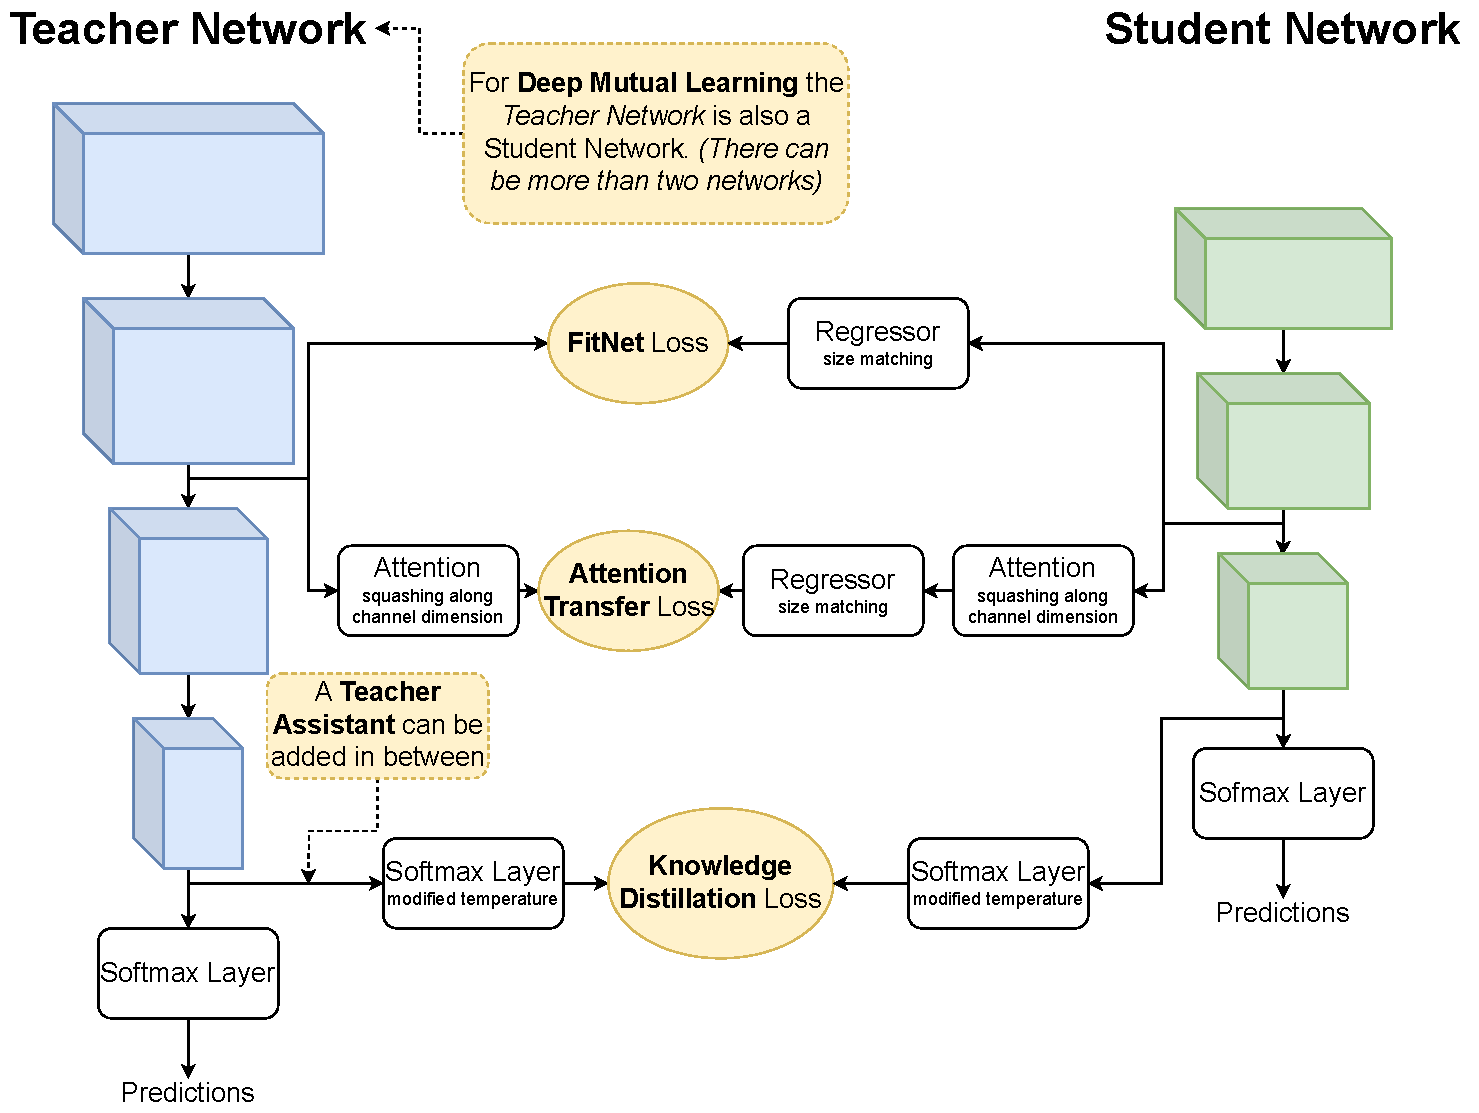
\includegraphics[width=0.75\textwidth]{chapter_sota/assets/kd_frameworks.pdf}
  \caption{Overview of various knowledge distillation frameworks. From top to
    bottom, left to right: Deep Mutual Learning
    \cite{DBLP:conf/cvpr/ZhangXHL18}, FitNet
    \cite{DBLP:journals/corr/RomeroBKCGB14}, Attention Transfer
    \cite{DBLP:conf/iclr/ZagoruykoK17}, Teacher Assistant
    \cite{DBLP:conf/aaai/MirzadehFLLMG20} and Knowledge Distillation
    \cite{DBLP:journals/corr/HintonVD15}.}
  \label{fig:sota:kd_frameworks}
\end{figure}

\subsection{Deep Mutual Learning}

Note that the aforementioned knowledge transfer methods require teacher-student
pairs and assume that teachers are large trained models.
\cite{DBLP:conf/cvpr/ZhangXHL18} relax this assumption by proposing \emph{Deep
Mutual Learning}, which enables a pool of networks of different architectures to
learn together, provided that they have the same logit dimensions, and none of
the models in the pool requires a pretraining step. The uncertainty of each
model is distilled into each other, which creates additional knowledge.\\

\subsection{Teacher Assistant}
In all the aforementioned methods, the efficacy of knowledge distillation, and
consequently, the final performance of the student network, is significantly
influenced by the disparity in size between the student and teacher networks.
This size discrepancy, when excessive, may cause the student network to
encounter difficulties in aligning with the teacher logits, thus preventing
optimal knowledge distillation. To tackle this issue,
\citeauthor{DBLP:conf/aaai/MirzadehFLLMG20} introduced the concept of
\emph{Teacher Assistant}: networks of intermediary dimensions aiming at bridging
the size gap between student and teacher \cite{DBLP:conf/aaai/MirzadehFLLMG20}.
The \ac{TA} approach proposes to ensure effective knowledge transfer through a
stepwise transfer of knowledge, starting from the teacher to the \ac{TA}, and
finally from the \ac{TA} to the student. This technique allows each model to
learn from a slightly simpler model than itself. Empirical evidence shows that
the \ac{TA} approach tends to outperform traditional one-step distillation in
various experiments and across different network architectures, resulting in
improved performances. However, it is important to note that it does introduce
additional computational overhead due to the necessity of additional training
steps for the \ac{TA}, and careful selection of the size and number of \acp{TA}.
These considerations underscore that while the \ac{TA} strategy is effective in
managing the size disparity problem, it also adds complexity to the distillation
process.\\


\begin{figure}[htbp]
  \centering
  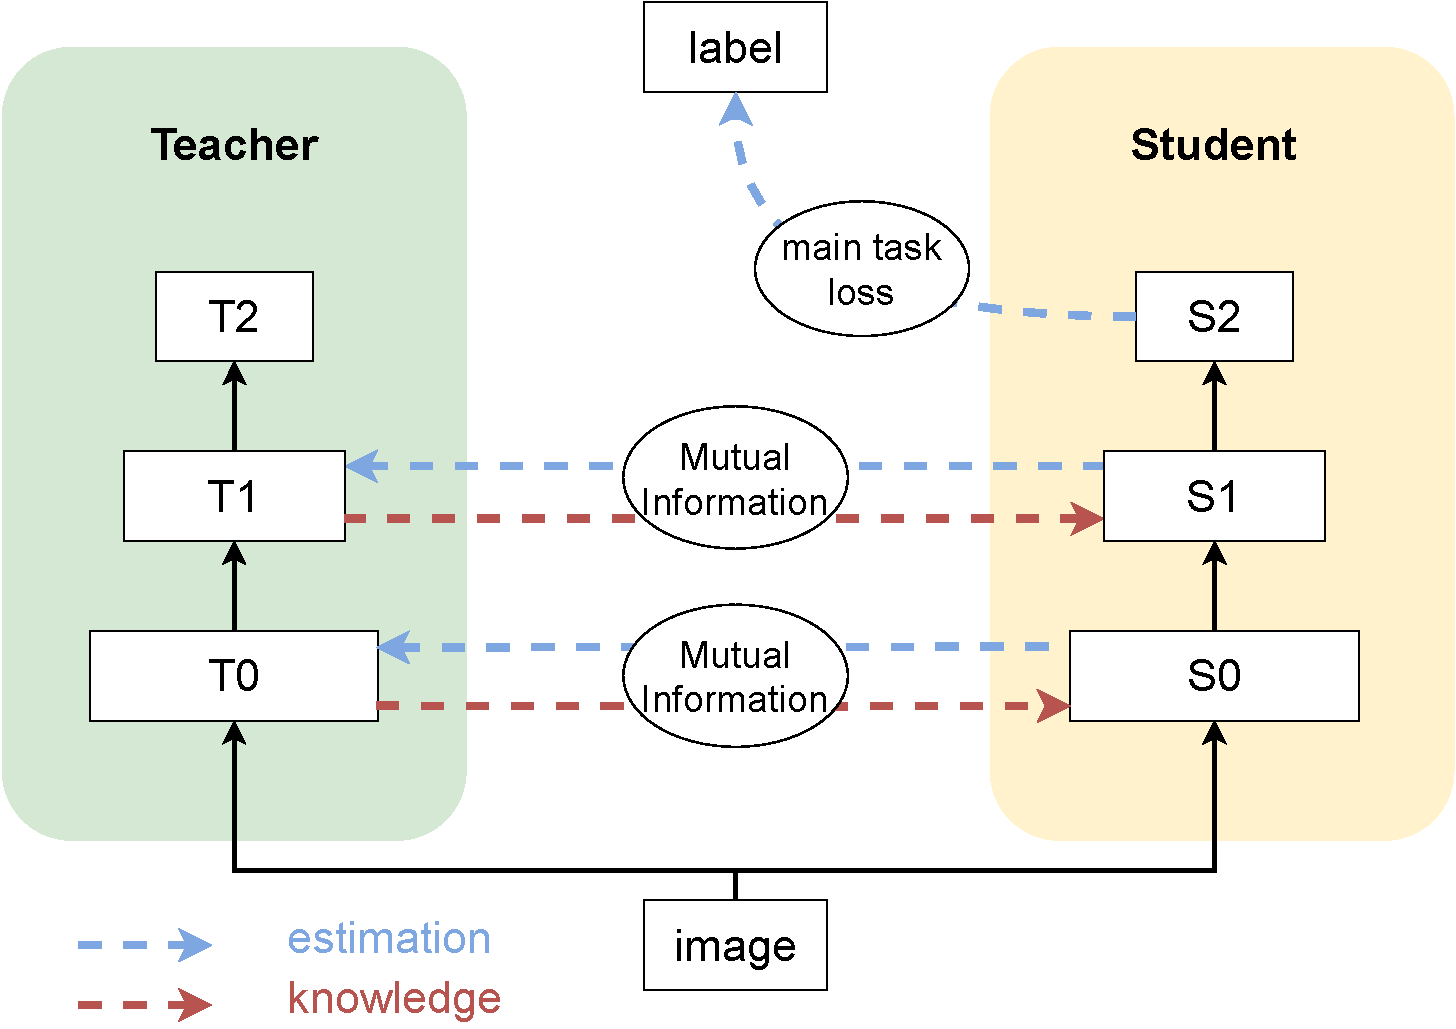
\includegraphics[width=0.7\textwidth]{chapter_sota/assets/variational_info_distillation.pdf}
  \caption{Conceptual scheme of \cite{DBLP:conf/cvpr/AhnHDLD19}. The student
    network efficiently learns the main task while retaining high mutual
    information with the teacher network. The mutual information is
    maximised by learning to estimate the distribution of the activations in
    the teacher network, provoking the transfer of knowledge. Adapted from
    the original scheme found in \cite{DBLP:conf/cvpr/AhnHDLD19}.}
  \label{fig:sota:vid_scheme}
\end{figure}

\subsection{Alternative Distillation Losses}
Other approaches that do not rely on direct feature map or logit matching have
been proposed. \cite{DBLP:conf/cvpr/AhnHDLD19} introduced \emph{Variational
  Information Distillation}, which indirectly maximises the mutual information
between the student and the teacher. This is done by using \emph{variational
  information maximisation} \cite{barber2004algorithm} to maximise a variational
lower bound of the mutual information, since directly maximising the latter is
intractable in practice (see \cref{fig:sota:vid_scheme}). Likewise,
\cite{DBLP:conf/eccv/PassalisT18} proposed a \emph{Probabilistic Knowledge
  Transfer} method that does not match logits or feature maps, but rather
represents the latter as a probability distribution and minimises divergence
between the two (see \cref{fig:sota:pkt_scheme}).\\


\begin{figure}[htbp]
  \centering
  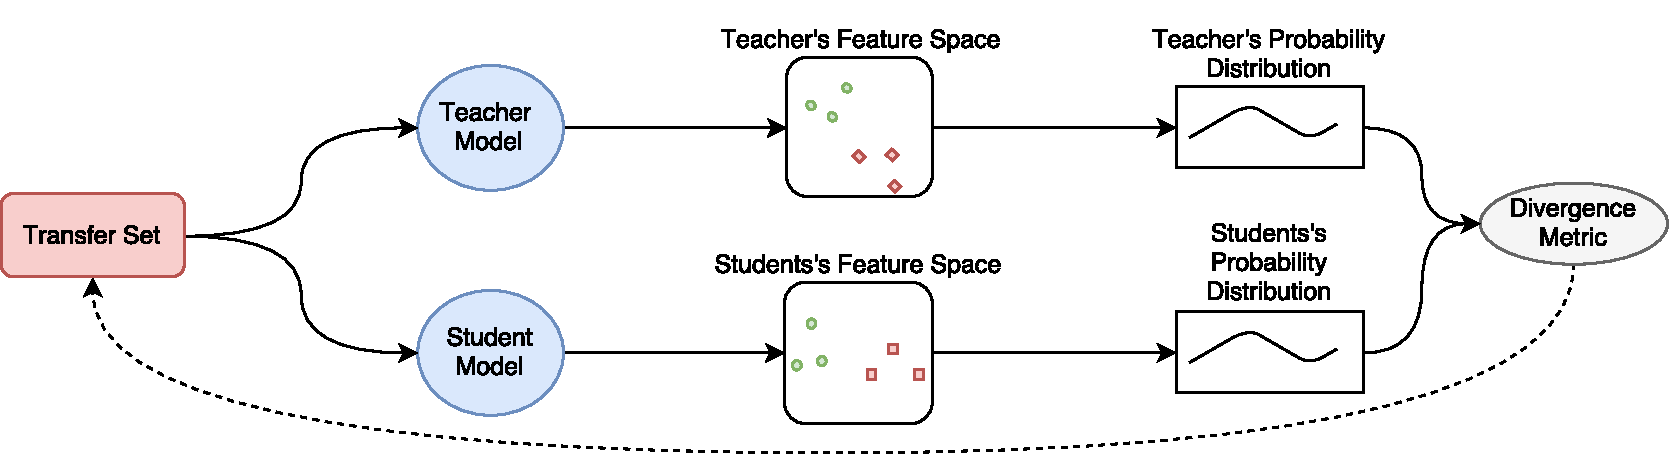
\includegraphics[width=0.7\textwidth]{chapter_sota/assets/pkt_diagram.pdf}
  \caption{Conceptual scheme of the Probabilistic Knowledge Transfer method.
    Both the student and the teacher feature maps are modelled using probability
    distributions. The divergence of the latter is minimised in order to
    transfer knowledge from the teacher to the student. Illustration taken from
    \cite{DBLP:conf/eccv/PassalisT18}.}
  \label{fig:sota:pkt_scheme}
\end{figure}

\section{Architecture Design}\label{sec:sota:archi_design}

The architectural design of neural networks, while contributing significantly to
their performance, often inflates their computational and memory requirements.
This increased complexity, although beneficial for the final performance, could
limit the deployment of these networks in resource-constrained environments.
Thus, formulating effective and efficient neural network architectures is of
significant importance. The design of neural networks is a problem that not only
involves designing suitable building blocks but also determining their
organization and interconnections. This section scrutinizes these aspects by
focusing on handmade and automatic efficient architecture design.\\

\Cref{sec:sota:efficient_archi} introduces building blocks to design efficient
architectures. These building blocks have been meticulously engineered in the
state-of-the-art to strike a balance between computational efficiency and
performance. Properly incorporating these blocks can result in architectures
better suited to their operating environments, enhancing efficiency while
maintaining the desired level of performance.\\

Thereafter, \cref{sec:sota:nas} delves into the field of \acl{NAS}. The primary
aim of \ac{NAS} is to design, in an automatic fashion, network architectures
that demonstrate a high level of efficiency and performance for a given task. By
doing so, it eliminates the need for manual design and the associated iterative
trial-and-error approaches that would otherwise be necessary to assess and
evaluate the impact and effectiveness of each design decision
\cite{DBLP:journals/corr/HowardZCKWWAA17,DBLP:conf/cvpr/SandlerHZZC18,DBLP:conf/iccv/HowardPALSCWCTC19}.
Although \ac{NAS} was not initially targeted at generating lightweight
architectures, the principles and methods described in this section can be
adapted to optimise the architecture search for efficiency and compactness. \\

This section explores techniques aimed at the creation of efficient and
effective neural networks through the careful selection and assembly of
optimised building blocks. The organization of these components plays an
important role in network compression and optimization, highlighting that high
performance can also be reached with designs that are less resource-demanding.\\

\subsection{Building Blocks for Efficient Architecture Design}\label{sec:sota:efficient_archi}
% region: depthwise separable convolutions

\textbf{Depthwise Separable Convolutions.} One of the initial strategies towards
achieving efficiency in neural network architectures is the use of depthwise
separable convolutions. This technique, used in MobileNet
\cite{howard2017mobilenets} and EfficientNet \cite{DBLP:conf/icml/TanL19},
separates the standard convolution operation into two distinct steps: a
depthwise convolution and a pointwise convolution (see
\cref{fig:sota:depthwise_conv_vs_standard_conv}). By decomposing the operations
in this manner, the computational complexity is markedly reduced while still
retaining the ability to capture spatial and channel-wise information. Consider
an input feature map with $C_\text{in}$ channels of arbitrary width and height
and $C_\text{out}$ convolution kernels of size $k\times k \times C_\text{in}$. A
standard convolution algorithm will need $C_\text{in} \times C_\text{out} \times
  k \times k$ \ac{MAC} operations to produce a $1 \times 1 \times C_\text{out}$
element of the output feature map. In contrast, a depthwise separable
convolution algorithm will first apply a $k\times k \times 1$ convolution kernel
to the $C_\text{in}$ channels and then perform $C_\text{out}$ pointwise
convolutions with $1\times 1 \times C_\text{in}$ kernels to produce the same
$1\times 1 \times C_\text{out}$ element. This effectively reduces the number of
parameters to $C_\text{in} \times (C_\text{out} + k \times k)$, essentially
reducing the number of computations required to produce a $1 \times 1 \times
  C_\text{out}$ element by a factor of\\

$$\displaystyle\frac{C_\text{out}\times k \times k}{C_\text{out} + k \times k}.$$\\

\begin{figure}[htbp]
  \centering
  \subfloat[Standard Convolution\label{fig:sota:standard_convolution}]{
    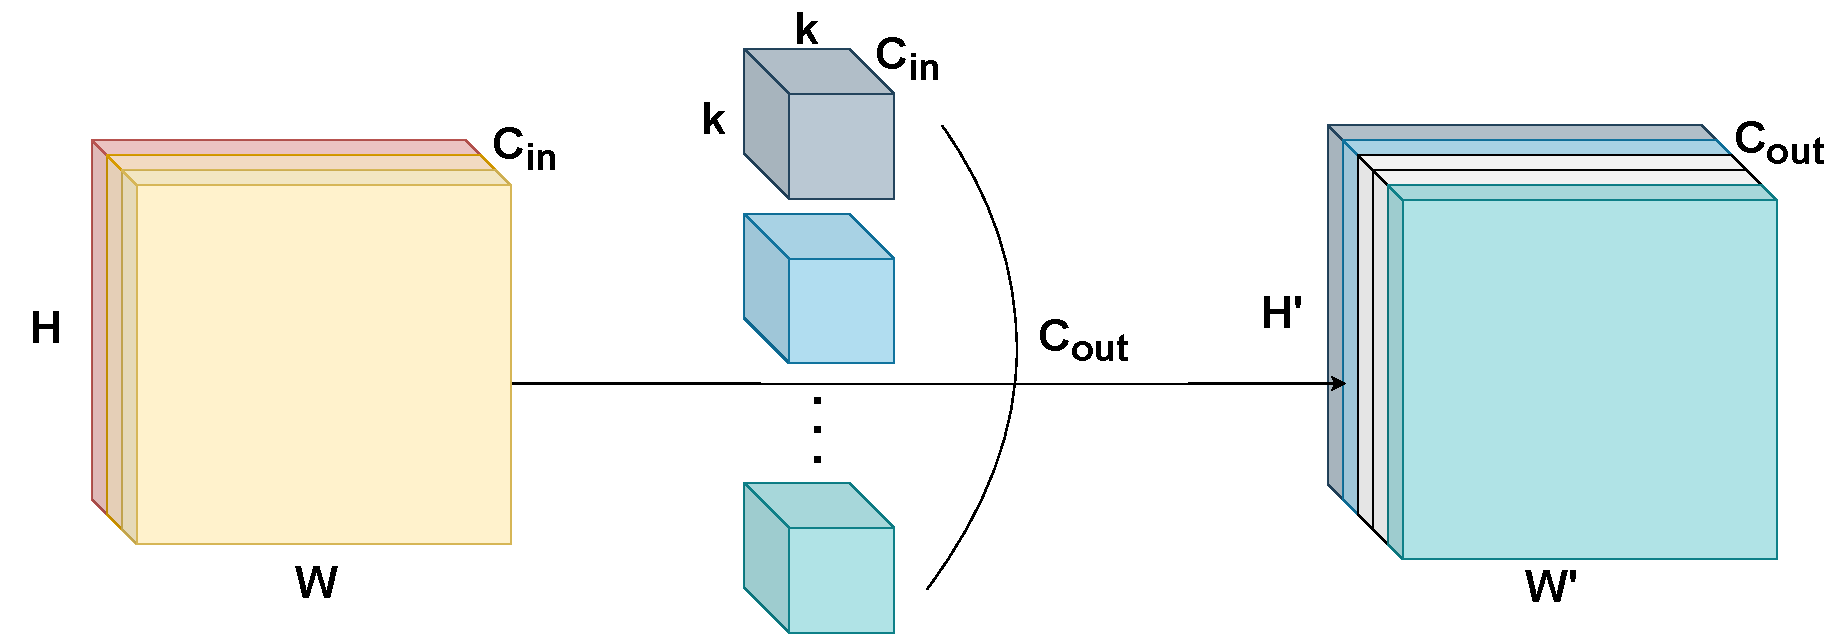
\includegraphics[width=0.70\textwidth]{chapter_sota/assets/standard_conv_scheme.pdf}}\\
  \vspace{1cm}
  \subfloat[Depthwise Separable
    Convolution\label{fig:sota:depthwise_convolution}]{
    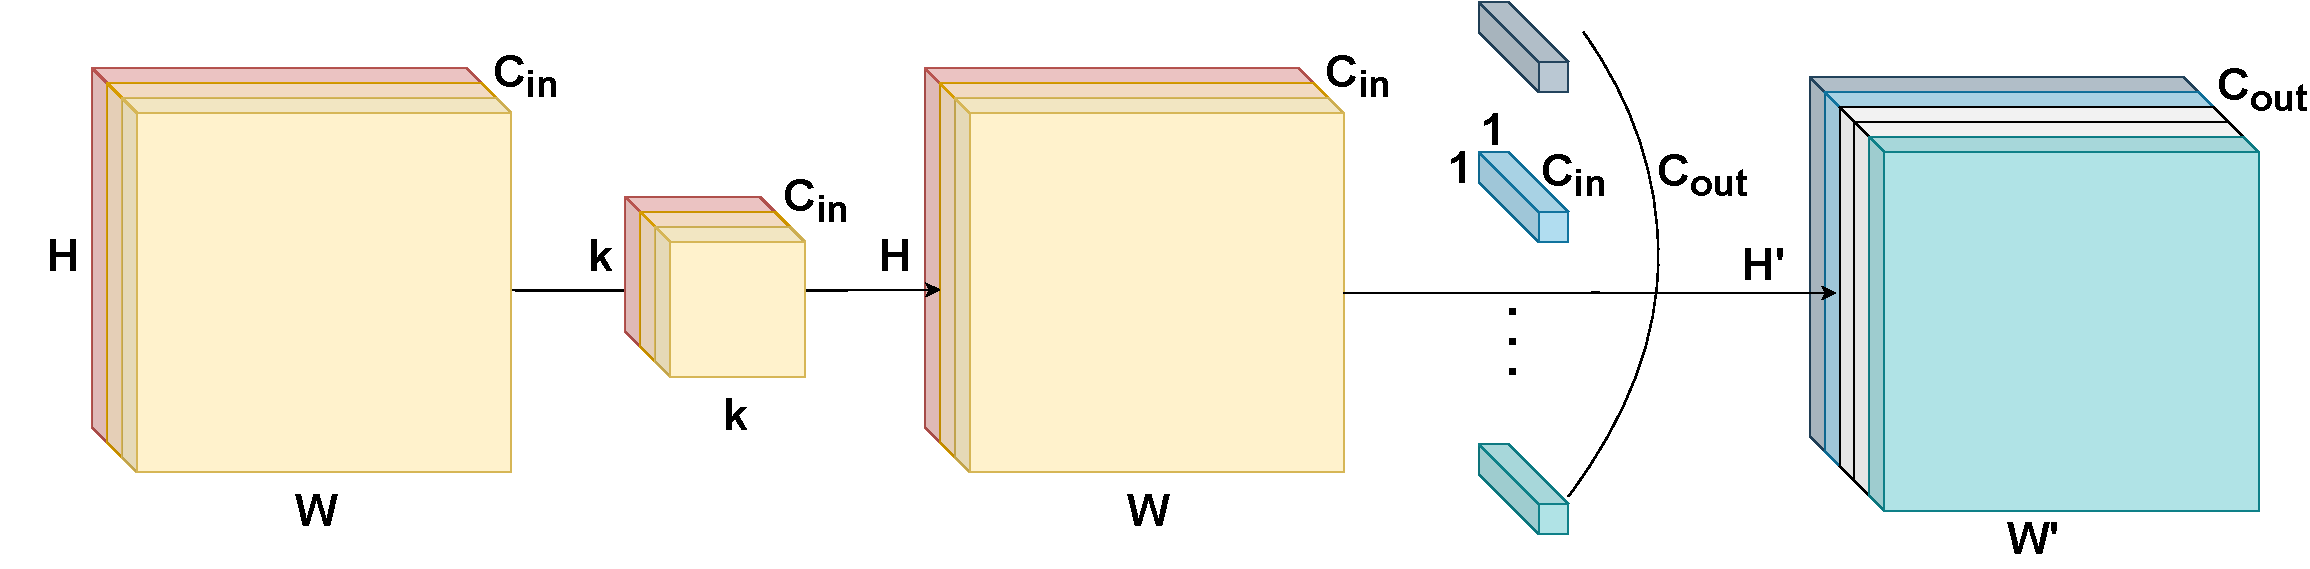
\includegraphics[width=0.70\textwidth]{chapter_sota/assets/depthwise_sep_conv_scheme.pdf}}
  \caption{Illustration schemes of the standard and depthwise separable
    convolution. The standard convolution uses $C_\text{out}$ kernels of size
    $k\times k \times C_\text{in}$. The depthwise separable convolution is
    split into two steps: \emph{(i)} a convolution with $C_\text{in}$ kernels
    of size $k \times k$ and \emph{(ii)} a convolution with $C_\text{out}$
    kernels of size $1\times 1 \times C_\text{in}$.
    Best viewed in colours.}
  \label{fig:sota:depthwise_conv_vs_standard_conv}
\end{figure}

% endregion: depthwise separable convolutions

% region: fire module
\noindent \textbf{Fire Module.} An alternative approach for designing efficient
architectures involves the integration of \emph{fire modules}, as proposed in
\cite{DBLP:journals/corr/IandolaMAHDK16}. These modules, represented in
\cref{fig:sota:fire_module}, aim to minimise computational requirements by
employing two distinct strategies: \emph{(i)} diminishing the number of input
channels supplied to the following conventional $k\times k$ convolutions and
\emph{(ii)} substituting a portion of the resource-intensive $k\times k$
convolutions with pointwise convolutions, which possess $k^2$ times fewer
parameters. The initial strategy is applied within the \emph{Squeeze Layer} of
the \emph{fire module}, which decreases the number of input channels delivered
to the \emph{Expand Layer}, subsequently reducing the number of parameters in
the \emph{Expand Layer} kernels. The second strategy is implemented in the
\emph{Expand Layer}, where some $3\times3$ convolutions are replaced with
$1\times1$ variants. Although the $1\times1$ convolutions capture less spatial
information, they are significantly less computationally demanding than the
$3\times3$ ones.\\

\begin{figure}[htbp]
  \centering
  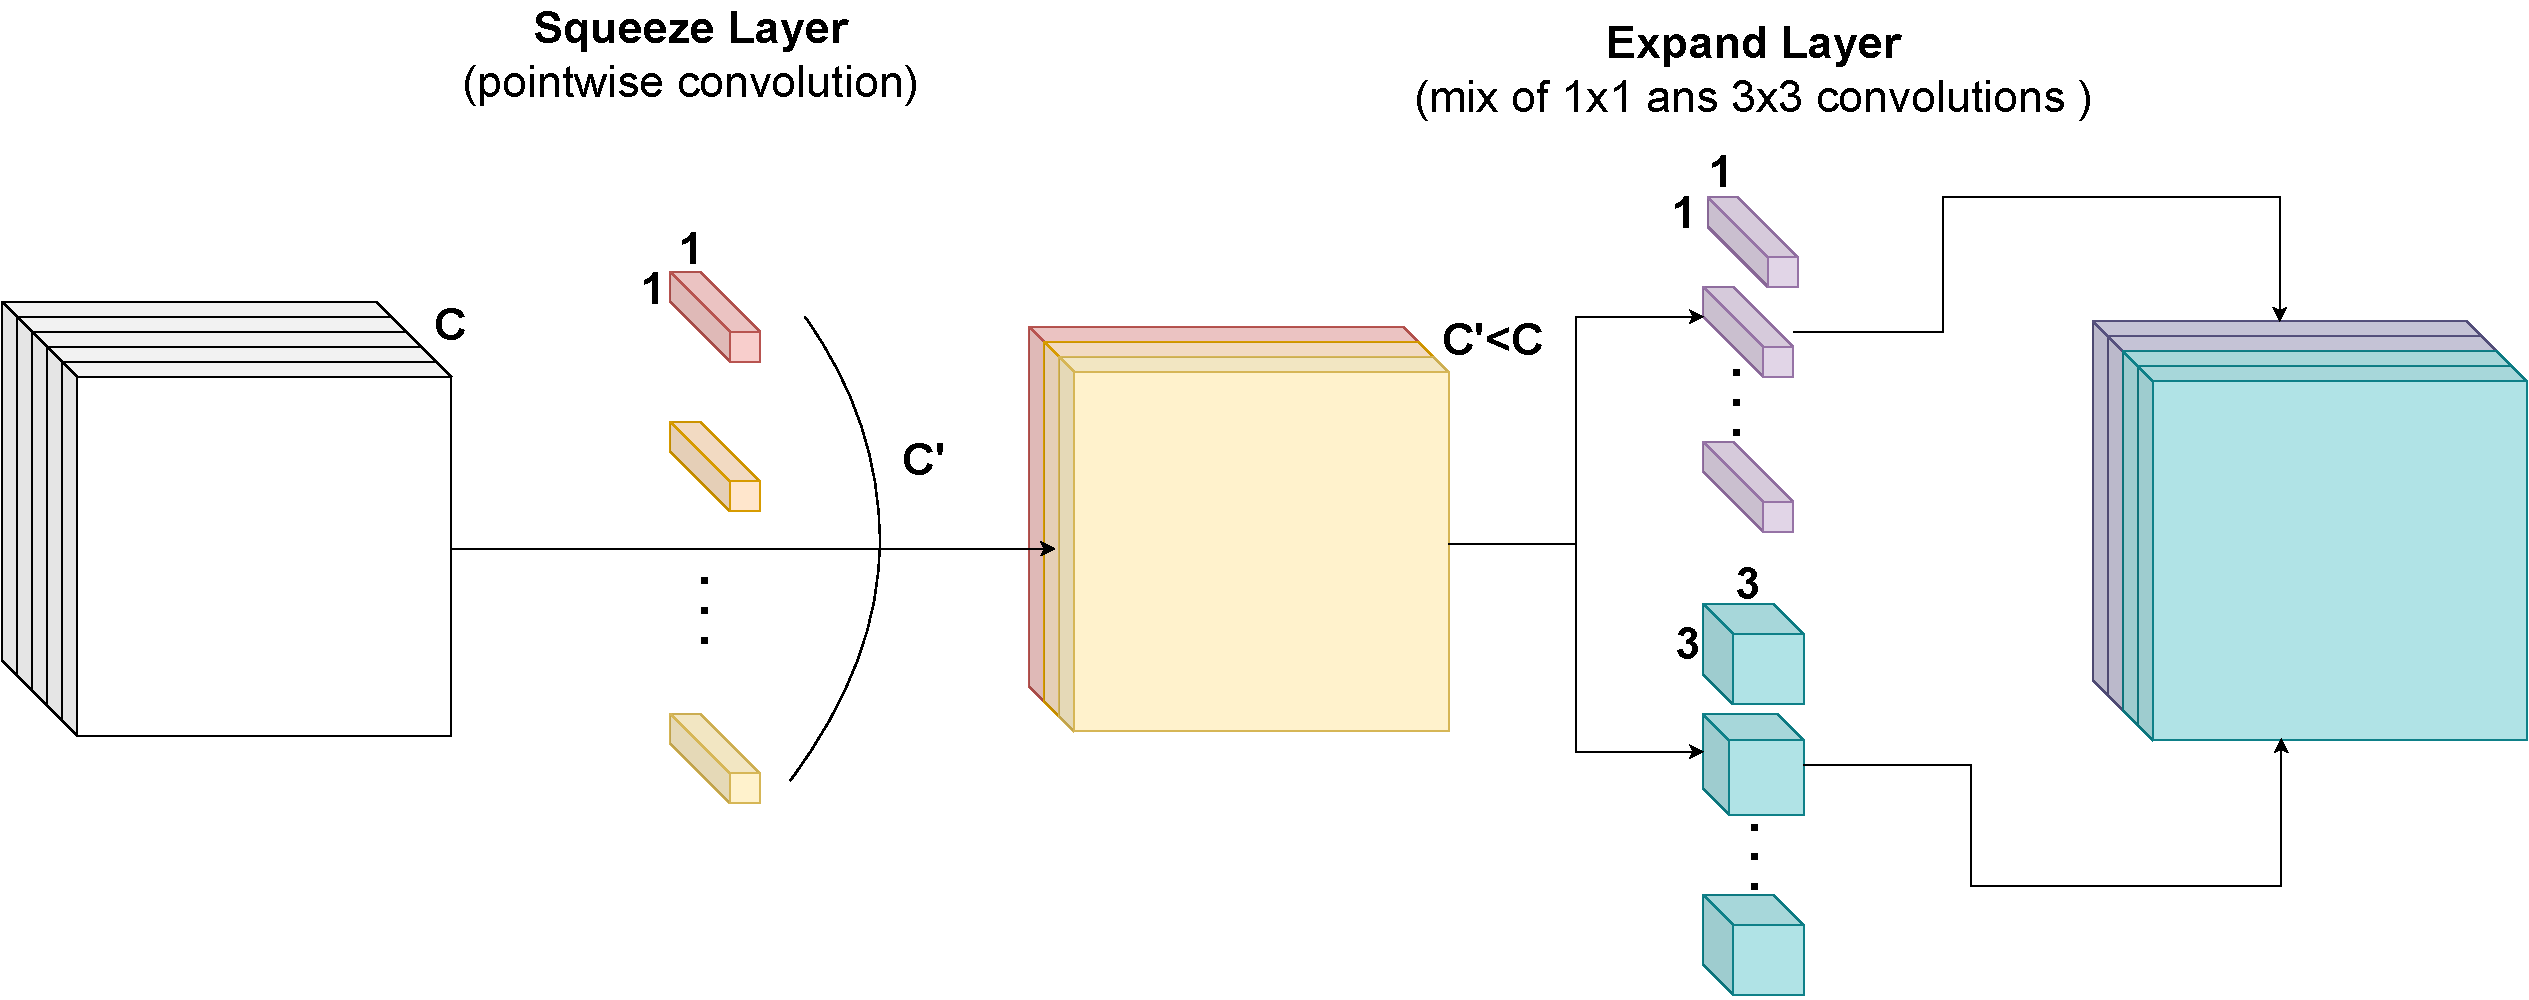
\includegraphics[width=0.70\textwidth]{chapter_sota/assets/fire_module.pdf}
  \caption{Illustration scheme of the fire module. The fire module is composed
    of a \emph{squeeze layer} (pointwise convolution designed to reduce the
    number of channels fed to the following layer) and an \emph{expand layer}
    (convolution with mixed $1\times1$ and $3\times3$ kernels. The $1\times1$
    kernels replace some of the $3\times3$ kernels, being less computationally
    intensive.). Best viewed in colours.}
  \label{fig:sota:fire_module}
\end{figure}

% endregion: fire module

% region: shufflenet

\noindent\textbf{ShuffleNet.} Pushing the concept of depthwise separable
convolutions further, \cite{ZhangShuffleNet} introduces pointwise group
convolutions and channel shuffle operations to enhance efficiency while
maintaining accuracy. Pointwise group convolutions were initially introduced in
\cite{DBLP:conf/nips/KrizhevskySH12}, though their original purpose was not for
compression. Instead, group convolutions in \cite{DBLP:conf/nips/KrizhevskySH12}
were used to enable distributed training across multiple \acp{GPU} with limited
memory. However, ShuffleNet \cite{ZhangShuffleNet} leverages this concept for
network efficiency by dividing the input channels into groups and performing
convolutions on each group independently. This approach reduces the number of
operations and the computational cost compared to traditional convolutions. To
counteract the potential loss of expressive power caused by the separation of
channels into groups, ShuffleNet incorporates \emph{channel shuffle operations}
as shown in \cref{fig:sota:shuffle_net}. This technique allows for information
exchange between groups, effectively maintaining accuracy by ensuring that
different groups can capture diverse features in the input.\\

\begin{figure}[htbp]
  \centering
  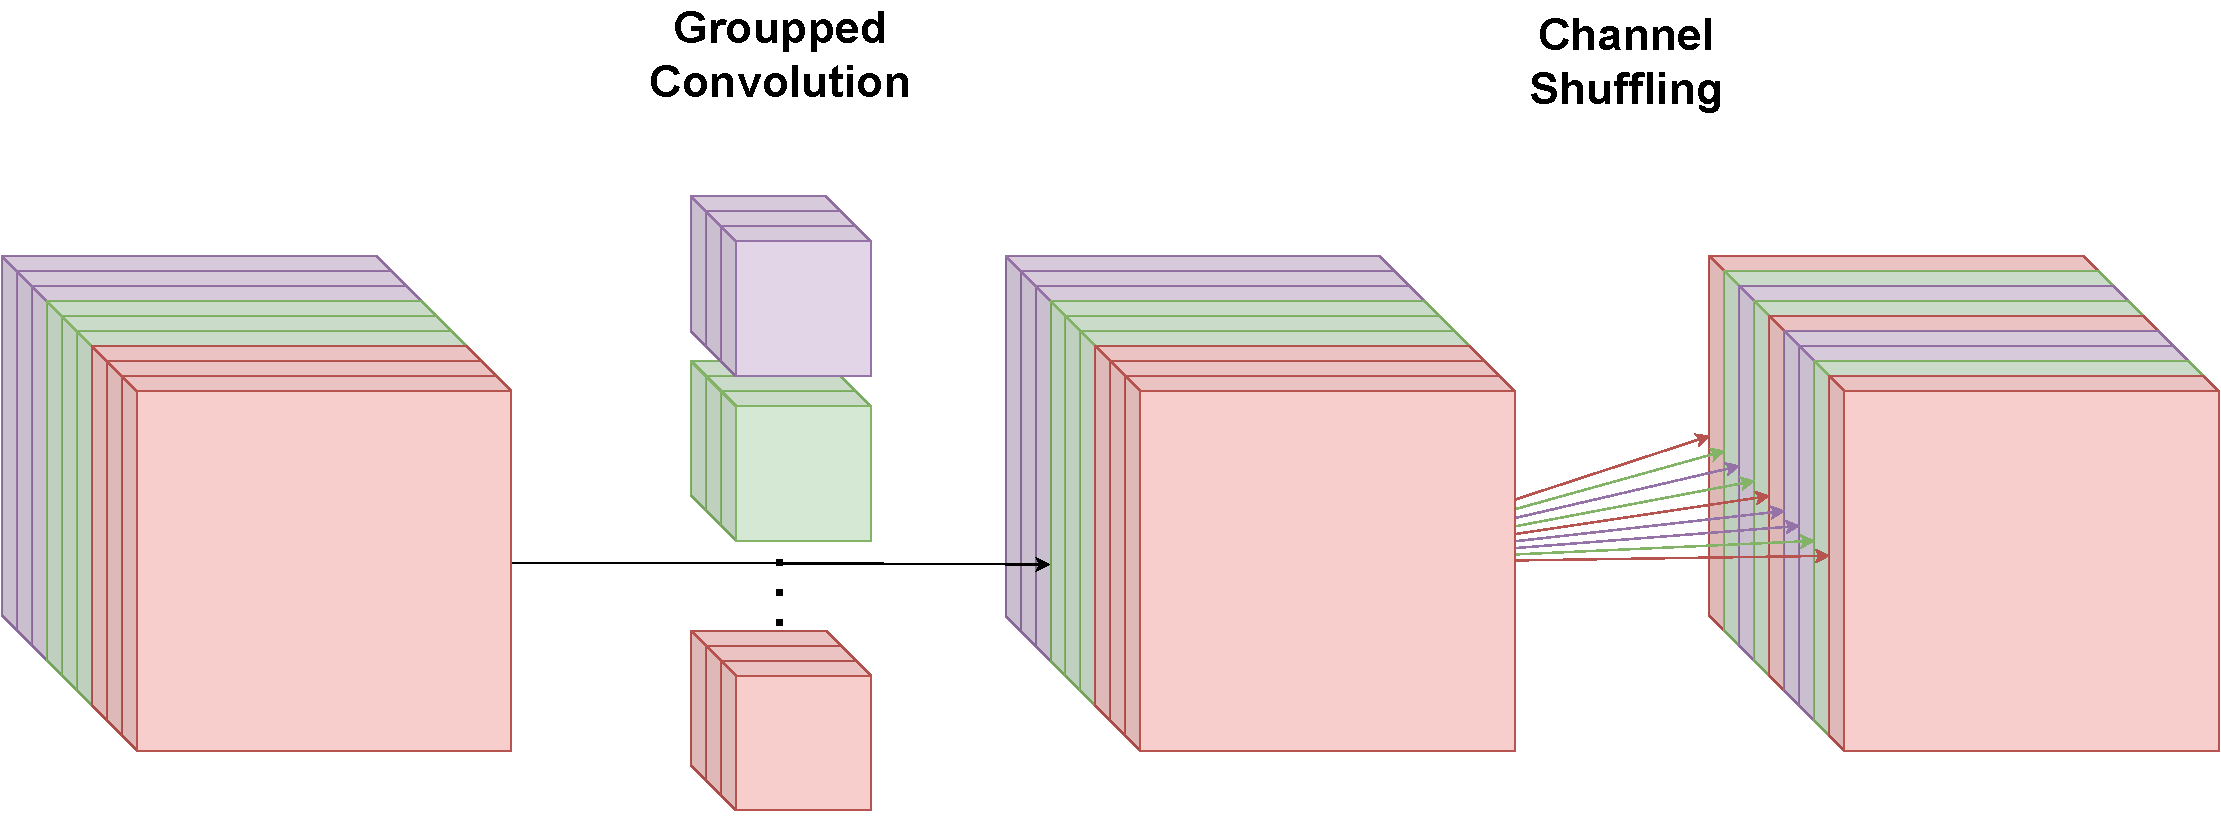
\includegraphics[width=0.70\textwidth]{chapter_sota/assets/group_conv_and_channel_shuffling.pdf}
  \caption{Illustration scheme of grouped convolution with channel shuffling.
    Each filter only acts on a subset of the input tensor (here represented by a
    matching colour). The channels of the yielded tensor are shuffled to ensure
    the subsequent groups can access information from all the previous groups.
    Best viewed in colours.}
  \label{fig:sota:shuffle_net}
\end{figure}

\noindent\textbf{Learned group convolutions.} Following ShuffleNet, CondenseNet was
introduced in \cite{huang2018condensenet},
incorporating learned group convolutions to further enhance efficiency. Unlike
the predefined group convolutions in ShuffleNet, CondenseNet learns which
channels should be grouped together, enabling the network to adapt its structure
for a specific task. This results in better utilisation of network capacity and
reduces redundancy. CondenseNet leverages the DenseNet architecture
\cite{huang2017densely} to further improve performance. Thanks to the densely
connected architecture, features discarded in any layer can still be recovered
in subsequent ones.\\

\begin{figure}[htbp]
  \centering
  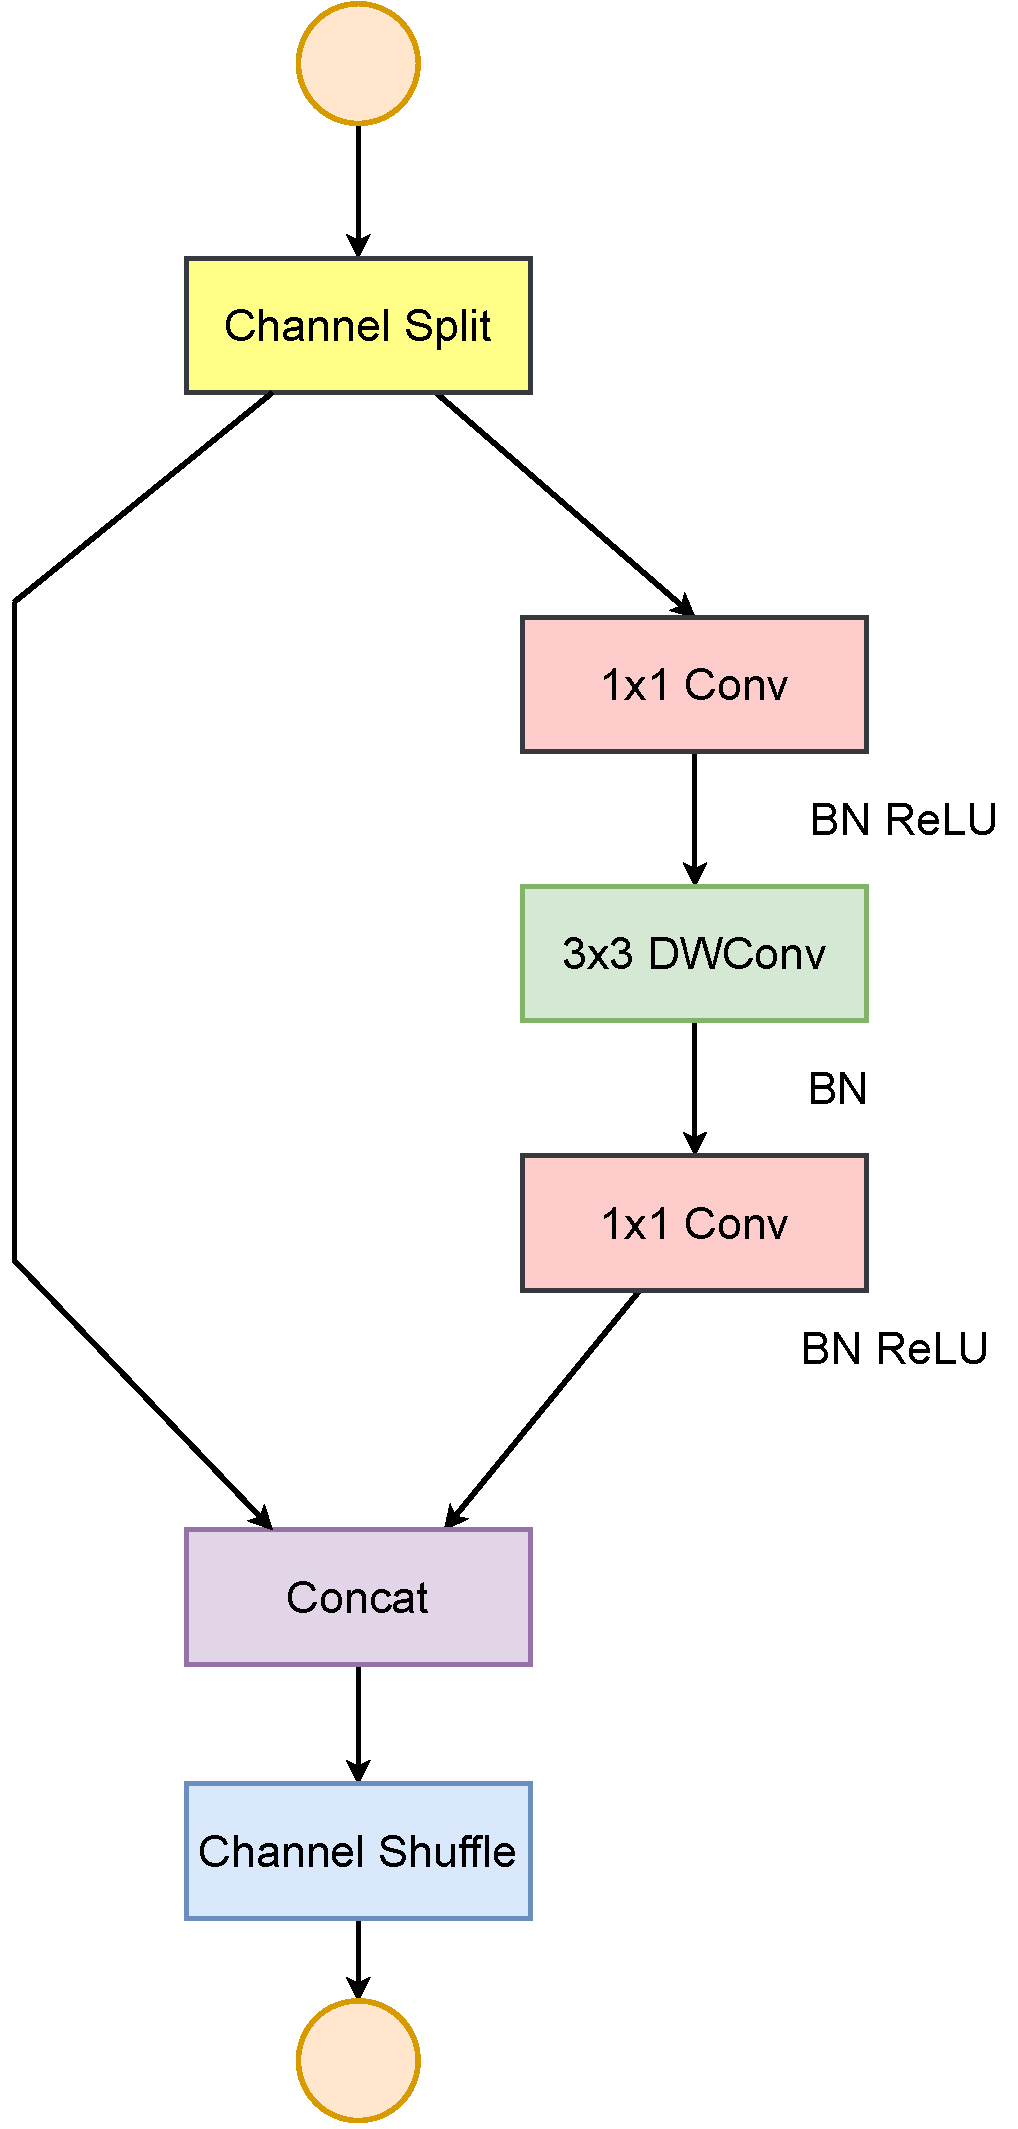
\includegraphics[width=0.7\textwidth]{chapter_sota/assets/channel_split.pdf}
  \caption{Illustration scheme of the path taken by the feature maps after the
    channel split block. Adapted from the original scheme found in \cite{MaShuffleNetV2}.}
  \label{fig:sota:channel_split}
\end{figure}

\noindent\textbf{ShuffleNetV2.} Building on the success of ShuffleNet,
ShuffleNetV2 was introduced in \cite{MaShuffleNetV2}, focusing on enhancing
network efficiency through the combination of strided convolution and channel
split. Strided convolution helps to reduce the spatial extent of feature maps,
thereby reducing the computation cost. The Channel Split technique efficiently
processes the input feature maps while maintaining the expressive power of the
architecture. Channel Split works by dividing the input feature maps into two
equal parts. One part is passed through the main branch of the ShuffleNet unit,
while the other part is sent through the identity branch, which leaves its input
unchanged. In the main branch, a sequence of pointwise and $3\times 3$
convolutions are performed. After both the main branch and the identity branch
complete their respective operations, the two parts are concatenated along the
channel dimension and the channels are shuffled. Finally, the output feature
maps are passed to the next ShuffleNet unit in the network. This process is
represented in \cref{fig:sota:channel_split}. This approach balances
computational efficiency with the expressive capacity of the model.\\
% endregion: shufflenet

% region: mobilenetv2
\noindent\textbf{Inverted residual and Linear bottlenecks.} Depthwise Separable
Convolutions were employed in MobileNet \cite{howard2017mobilenets}.
\citeauthor{DBLP:conf/cvpr/SandlerHZZC18} introduced skip connections and
residual blocks into the MobileNetV2 architecture
\cite{DBLP:conf/cvpr/SandlerHZZC18}, initially proposed in
\cite{DBLP:conf/cvpr/HeZRS16}. They also introduced the concept of inverted
residuals and linear bottlenecks. In conventional residual blocks, the input is
first compressed, then expanded, and finally compressed again after being added
to the original input. With inverted residual bottlenecks, on the other hand,
this process is reversed: the input is first expanded, then a depthwise
separable convolution is applied, and finally, it is compressed again. In this
architecture, the skip connections link the feature maps of smaller size,
instead of the larger ones. This allows for a more memory-efficient
architecture. The standard residual blocks and the inverted residual blocks are
shown in \cref{fig:sota:inverted_vs_residual_blocks}. The linear bottlenecks, on
the other hand, are convolutions with a linear activation function. This takes
advantage of the property that high-dimensional feature maps can be embedded in
a lower-dimensional manifold. To do this, it is necessary to use linear
transformations since non-linear ones could potentially destroy information as
reported in \cite{DBLP:conf/cvpr/SandlerHZZC18,DBLP:conf/cvpr/HanKK17}.\\

\begin{figure}[htbp]
  \centering
  \subfloat[Standard Residual Block\label{fig:sota:residual_block}]{%
    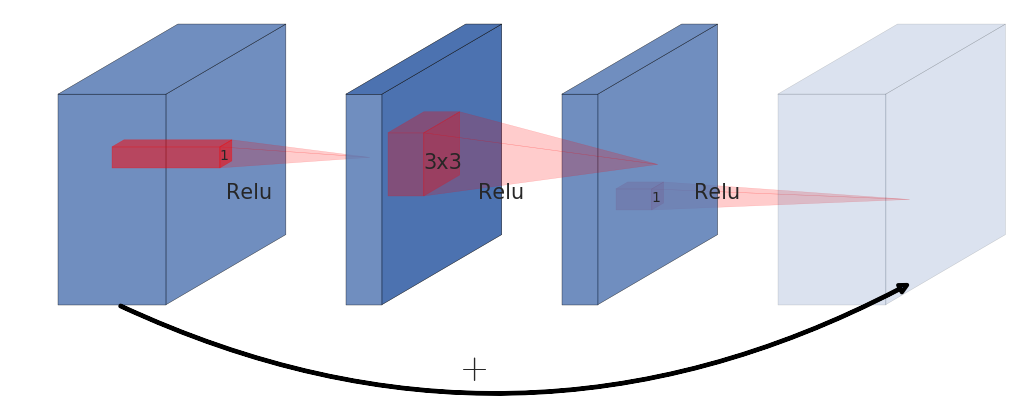
\includegraphics[width=0.49\textwidth]{chapter_sota/assets/mobilenet_v2_residual.png}}
  \subfloat[Inverted Residual Block\label{fig:sota:inverted_residual_block}]{%
    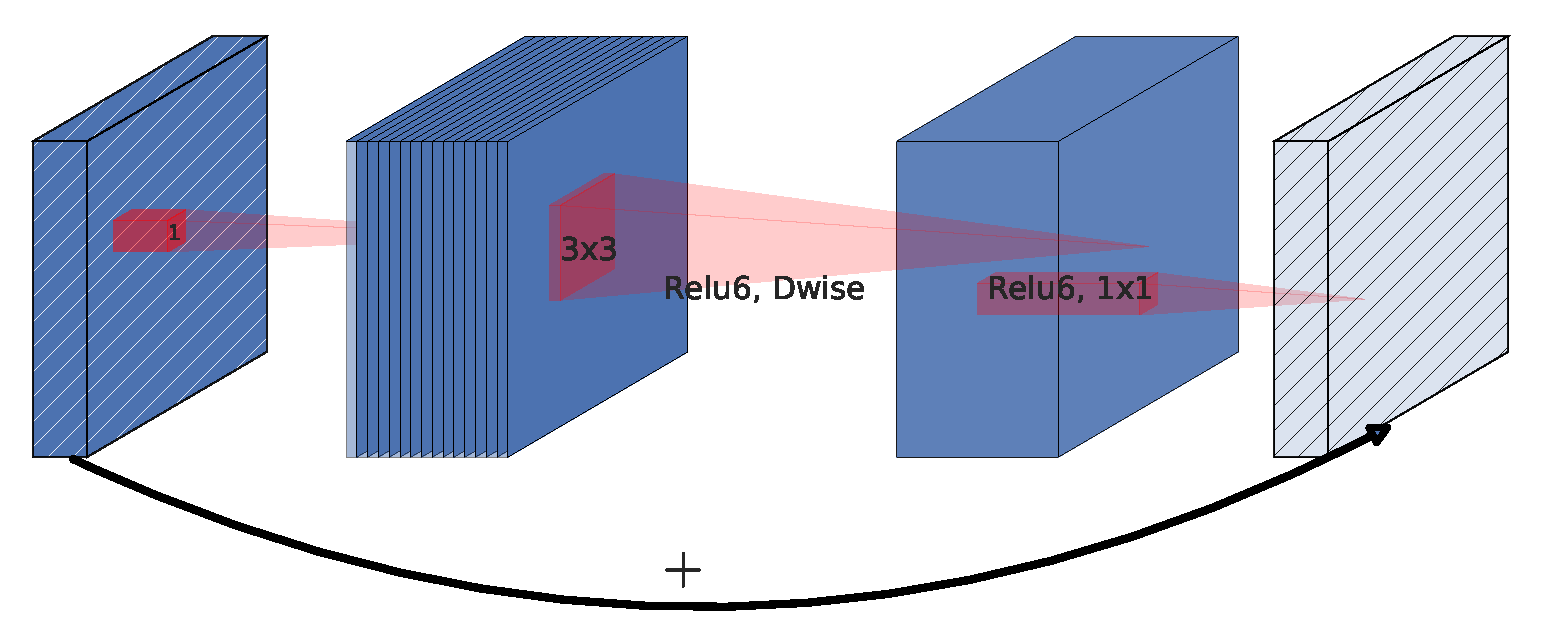
\includegraphics[width=0.49\textwidth]{chapter_sota/assets/mobilenet_v2_inverted_residual.pdf}}
  \caption{Illustration scheme of the residual block and the inverted residual
  block. Note that on the inverted residual block, the feature maps with the
  lower number of channels are the ones connected via the skip connection,
  whereas it is the opposite on the standard residual block. Diagonally hatched
  layers do not use non-linearities. The grey colour indicates the beginning of
  the next block. Both illustrations are taken from \cite{DongMobileNetV2}. Best
  viewed in colours.}
  \label{fig:sota:inverted_vs_residual_blocks}
\end{figure}

% endregion: mobilenetv2

% region: mobilenetv3
\noindent\textbf{Squeeze and excitation modules.} Advancing from MobileNet and
MobileNetV2, its third version \cite{DBLP:conf/iccv/HowardPALSCWCTC19}
incorporated \ac{SE} modules initially introduced in
\cite{DBLP:conf/cvpr/HuSS18}. These modules adaptively recalibrate channel-wise
feature responses, amplifying important features and suppressing less relevant
ones. The \ac{SE} module (represented in \cref{fig:sota:se_module}) performs
\emph{squeeze} and \emph{excitation} operations. The squeeze operation uses
global average pooling to create a channel descriptor that summarises the
spatial information for each channel. The excitation operation uses this
descriptor to learn non-linear interactions between channels through two fully
connected layers. The outputs of this mini-network are per-channel modulation
weights that recalibrate the original feature maps, scaling or "exciting" them
by these weights.\\

% endregion: mobilenetv3

\begin{figure}[htbp]
  \centering
  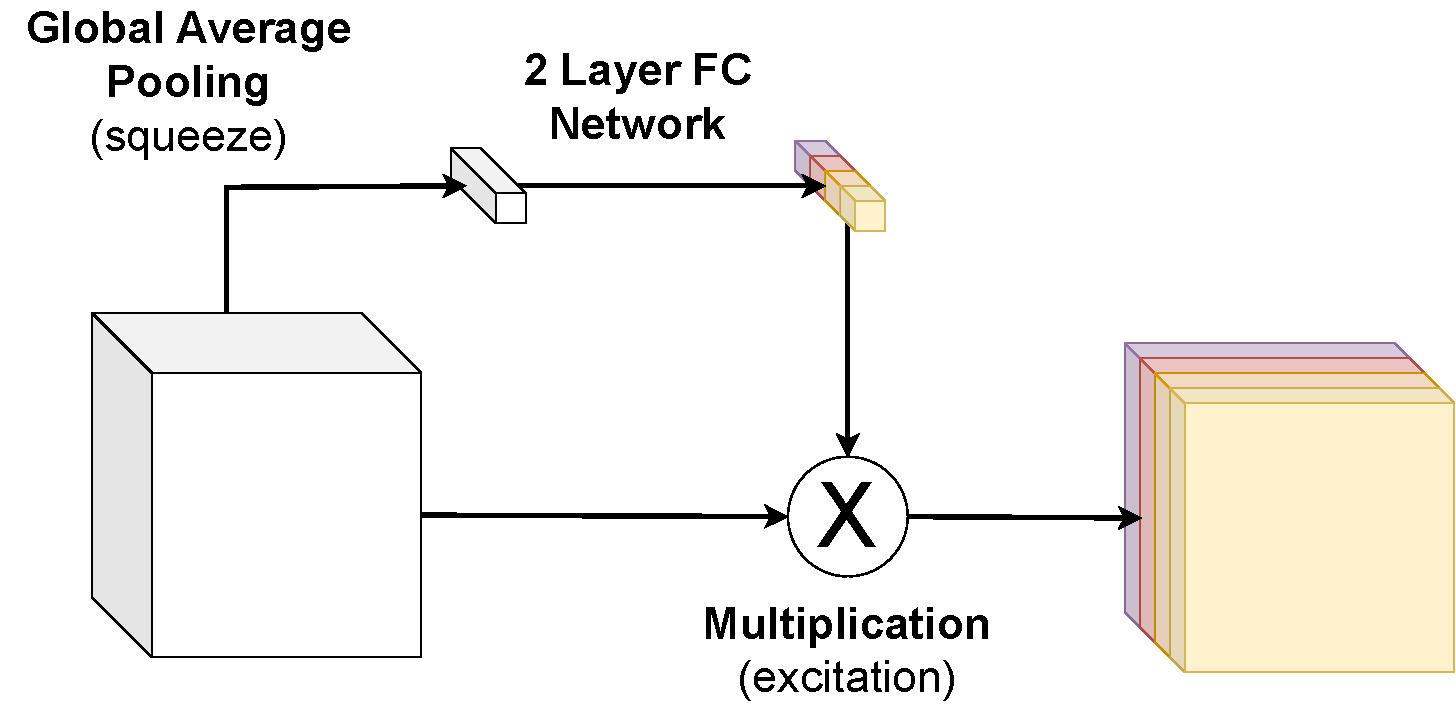
\includegraphics[width=0.70\textwidth]{chapter_sota/assets/SE_module.pdf}
  \caption{Illustration scheme of the \acf{SE} module. The original feature
    map is \emph{squeezed} into a channel descriptor through global average
    pooling. This descriptor is then used to learn the interdependencies between
    the channels through two fully connected layers. The output is then
    multiplied layerwise with the original feature map (\emph{excitation}). Best
    viewed in colours.}
  \label{fig:sota:se_module}
\end{figure}


% region: transition paragraph
The architectures we reviewed in this section revolve around specific key
techniques such as depthwise separable convolutions, fire modules, channel
shuffling, and \ac{SE} modules, among others. These architectures, while highly
efficient, are manually crafted and require a significant degree of human
expertise, intuition, and time to develop, optimise, and fine-tune. The manual
design of these architectures often relies on a deep understanding of the tasks
at hand, the data they will process, and the constraints of the environment in
which they will operate. However, the process of designing these efficient
architectures can be automated, which is the subject of the next section. Sizes
and performance of network architectures detailed in this section can be
compared to standard architecture sizes in \cref{fig:sota:net_sizes_std_eff}.\\

\begin{figure}[htbp]
  \centering
  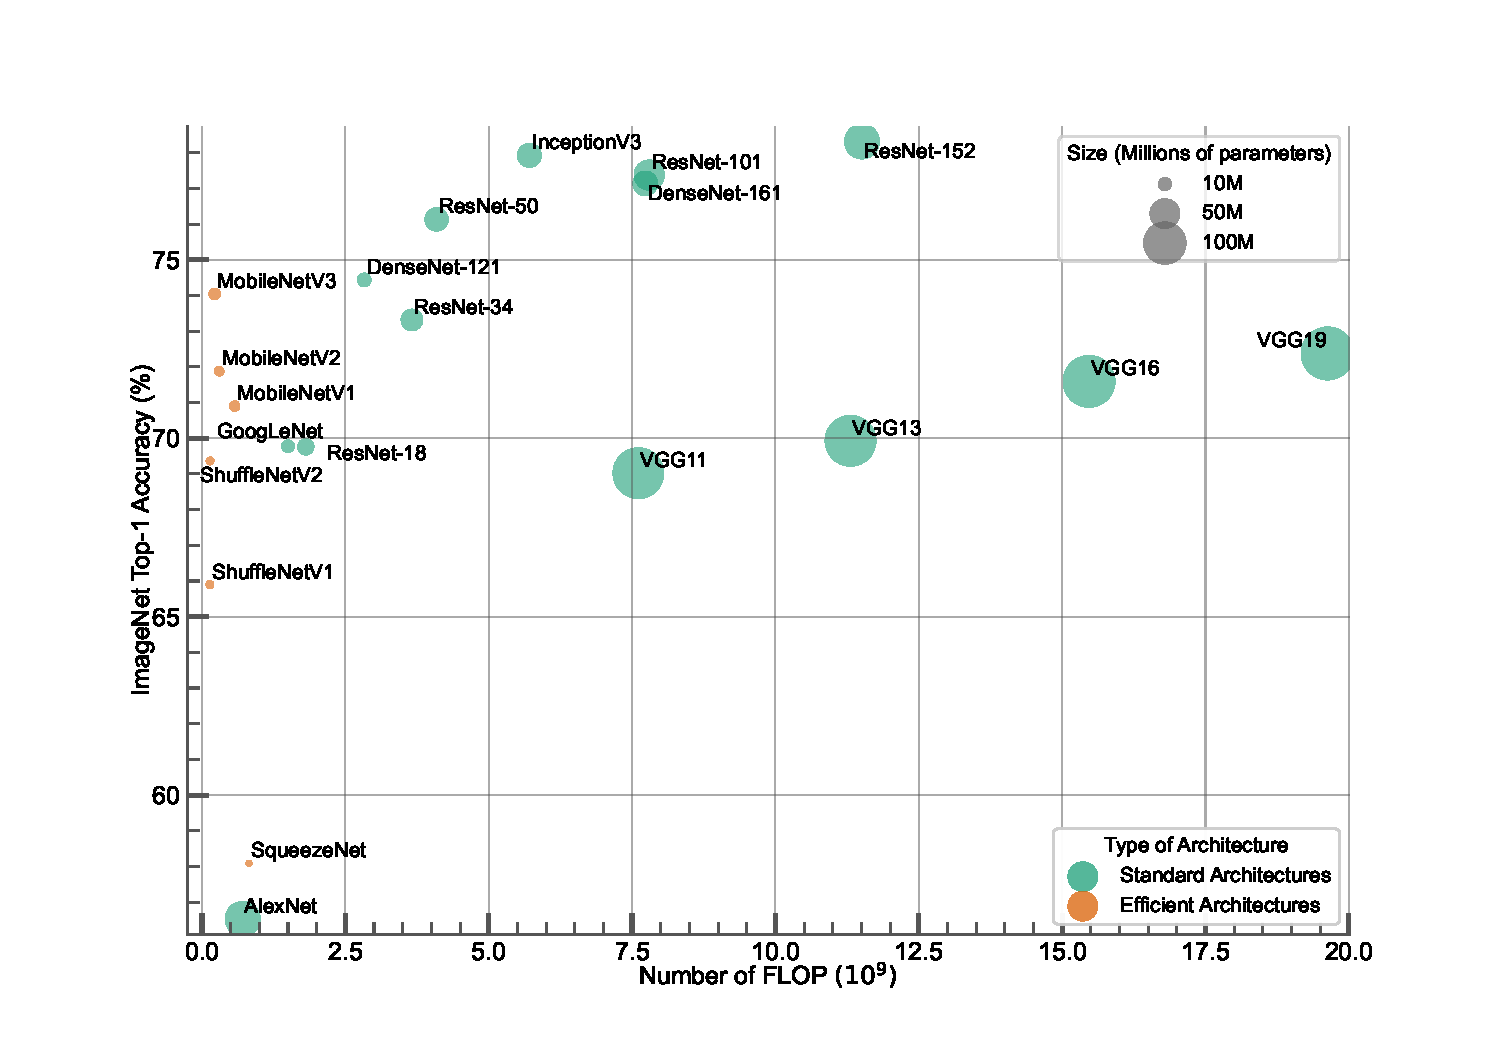
\includegraphics[width=0.70\textwidth]{chapter_sota/assets/network_sizes_normal_eff.pdf}
  \caption{\Cref{fig:dlo:net_sizes} updated with the size and performance of the
    efficient architectures detailed in \cref{sec:sota:efficient_archi}. Best
    viewed in colours.}
  \label{fig:sota:net_sizes_std_eff}
\end{figure}




% endregion: transition paragraph

\subsection{Automatic Architecture Design Through Neural Architecture Search}\label{sec:sota:nas}

\acf{NAS} is a method that automates the discovery of neural network
architectures, potentially leading to more compact, efficient designs and
reducing the need for manual intervention. Although \ac{NAS} might not
explicitly aim at producing lightweight architectures, it can still yield
designs that strike a good balance between performance and computational cost
\cite{DBLP:conf/cvpr/TanCPVSHL19,DBLP:conf/icml/TanL19}. By using automated
methods to search for optimal architectures, it is possible to further enhance
the efficiency of neural networks, opening up new possibilities for their
deployment in resource-constrained environments. \ac{NAS} has emerged as an
essential paradigm, aiming to automate the traditionally manual and
labour-intensive process of designing efficient neural networks
\cite{DBLP:journals/corr/MiikkulainenLMR17}. Early network architectures were
indeed entirely handcrafted, requiring significant human effort and expertise.
However, these manual methods are being replaced by \ac{NAS} techniques, which
seek to automatically determine the optimal network structure given a training
set \cite{DBLP:journals/corr/abs-2301-08727,elsken2019neural}.\\

The performance and efficiency of \ac{NAS} are fundamentally determined by two
key aspects: the \emph{search space} and the \emph{search strategy}. The search
space, as the name implies, defines the set of all possible architectures that
can be discovered by the \ac{NAS} algorithm. It could be as broad as all
possible configurations of a certain type of network, such as \acp{CNN}, or as
narrow as different arrangements of a specific set of layers
\cite{DBLP:conf/cvpr/LiuCSAHY019}. The search strategy, on the other hand,
determines how the \ac{NAS} algorithm navigates through this search space in
order to optimise its given objective. This could involve gradient-based
strategies \cite{DBLP:conf/iclr/LiuSY19,DBLP:conf/iclr/XuX0CQ0X20}, or
stochastic methods, such as evolutionary algorithms and reinforcement learning
\cite{DBLP:conf/iclr/ZophL17,DBLP:conf/icml/RealMSSSTLK17}. The choice of search
space and search strategy significantly influences the ability of \ac{NAS} to
discover effective and efficient architectures and is thus a critical aspect of
NAS research. In the following paragraphs, we will delve deeper into some of the
major strategies and their impact on the field of \ac{NAS}.\\



\noindent\textbf{Search space.} The search space is a critical aspect of
\ac{NAS} as it bounds the possibilities of architectures and significantly
influences the outcome of the search. The search space could be as broad as all
possible configurations of a certain network type or as specific as various
arrangements of a predefined set of layers or blocks. For instance,
\cite{DBLP:conf/iclr/ZophL17} define their search space as a set of repeatable
sub-structures composed of basic layers (convolution layers, fully connected
layers, \ac{BN} layers, etc...) often called \emph{cells} that are stacked to
form the final architecture, while \cite{DBLP:conf/iclr/XieZLL19} design their
search space based on the connectivity patterns between network blocks. DARTS
\cite{DBLP:conf/iclr/LiuSY19} propose a continuous search space where the
architecture is parameterized as a differentiable function, allowing for
efficient search using gradient-based methods. Hierarchical search spaces, on
the other hand, offer a strategic approach which allows to manage the complexity
of the architecture search in \ac{NAS}
\cite{DBLP:conf/cvpr/LiuCSAHY019,DBLP:conf/cvpr/TanCPVSHL19}. In such a setup,
the architecture is divided into several levels of hierarchy, with each one
searched independently. This structure enables a more systematic and organized
exploration of the search space, allowing the algorithm to uncover useful
patterns and configurations at different levels of the network. The EfficientNet
models are exemplary of innovative architecture search strategies
\cite{DBLP:conf/icml/TanL19}. This series utilizes both \ac{NAS} and
\emph{compound scaling}. A baseline, EfficientNet-B0, was developed through
multi-objective \ac{NAS}, optimizing both accuracy and \acp{FLOP}. Subsequently,
a compound scaling method was applied to this baseline, uniformly scaling depth,
width, and resolution via a \emph{compound coefficient}. This approach yielded a
series of progressively larger EfficientNet models, whose performances are shown
in \ref{fig:sota:efficientnet_perfs}.\\\


\begin{figure}[htbp]
  \centering
  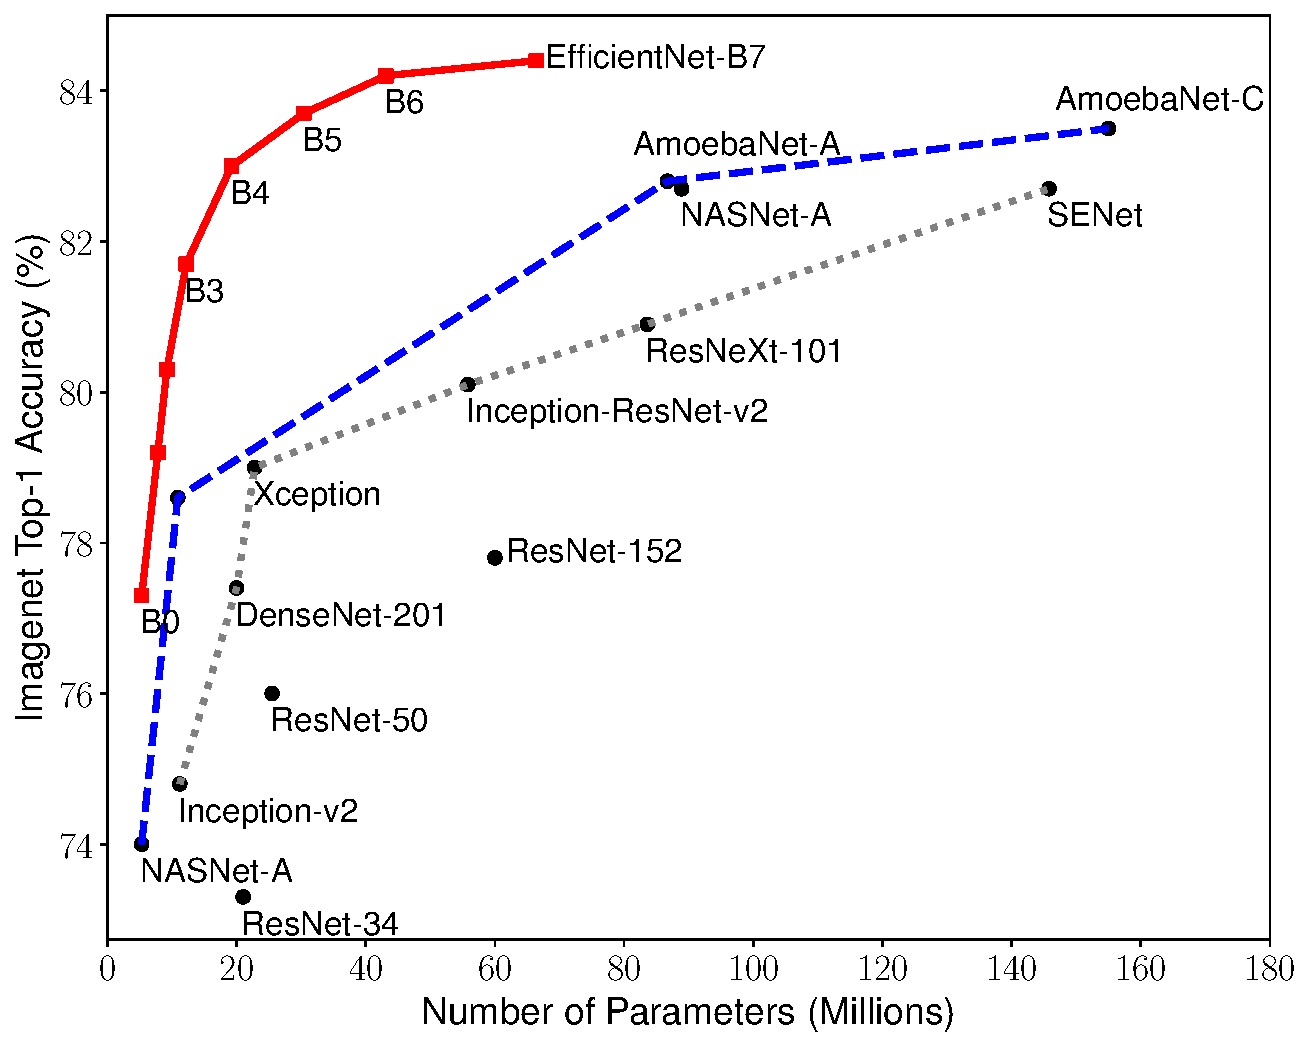
\includegraphics[width=0.70\textwidth]{chapter_sota/assets/efficientnet_perfs_overview.pdf}
  \caption{ImageNet top-1 accuracy vs model size (in millions of parameters).
    The EfficientNet family of models significantly outperforms other models of
    similar size, obtained either by \ac{NAS} or manual design. This graph is
    taken from \cite{DBLP:conf/icml/TanL19}.
  }
  \label{fig:sota:efficientnet_perfs}
\end{figure}


\noindent\textbf{Search strategy.} The search strategy is another major
component of \ac{NAS}, dictating how the algorithm explores the search space to
find the optimal architecture. A wide range of search strategies have been
proposed. Evolutionary algorithms \cite{DBLP:conf/icml/RealMSSSTLK17} use
principles of natural evolution such as mutation, crossover, and selection to
explore the search space. Despite their potential to find high-quality
solutions, these methods often require substantial computational resources due
to the large number of evaluations needed. Reinforcement Learning-based methods
\cite{DBLP:conf/iclr/ZophL17} employ a policy network to generate architectures
and a reward signal, typically validation accuracy, to guide the search. While
reinforcement learning methods can effectively navigate large search spaces,
their success heavily depends on the quality of the reward signal.
Gradient-based methods \cite{DBLP:conf/iclr/LiuSY19,DBLP:conf/iclr/XuX0CQ0X20}
make the search space continuous and use gradient descent for optimization,
which enables efficient exploration of the search space but requires careful
regularization to prevent overfitting. \cite{DBLP:conf/nips/BergstraBBK11} uses
Bayesian optimization to build a probabilistic model of the objective function
and uses it to select promising architectures, balancing exploitation and
exploration. This method can be sample-efficient but might struggle with
high-dimensional spaces. These diverse strategies offer multiple paths to
navigate the complex landscape of architecture search, each with its unique
trade-offs between efficiency, effectiveness, and computational demands.\\


\begin{figure}[htbp]
  \centering
  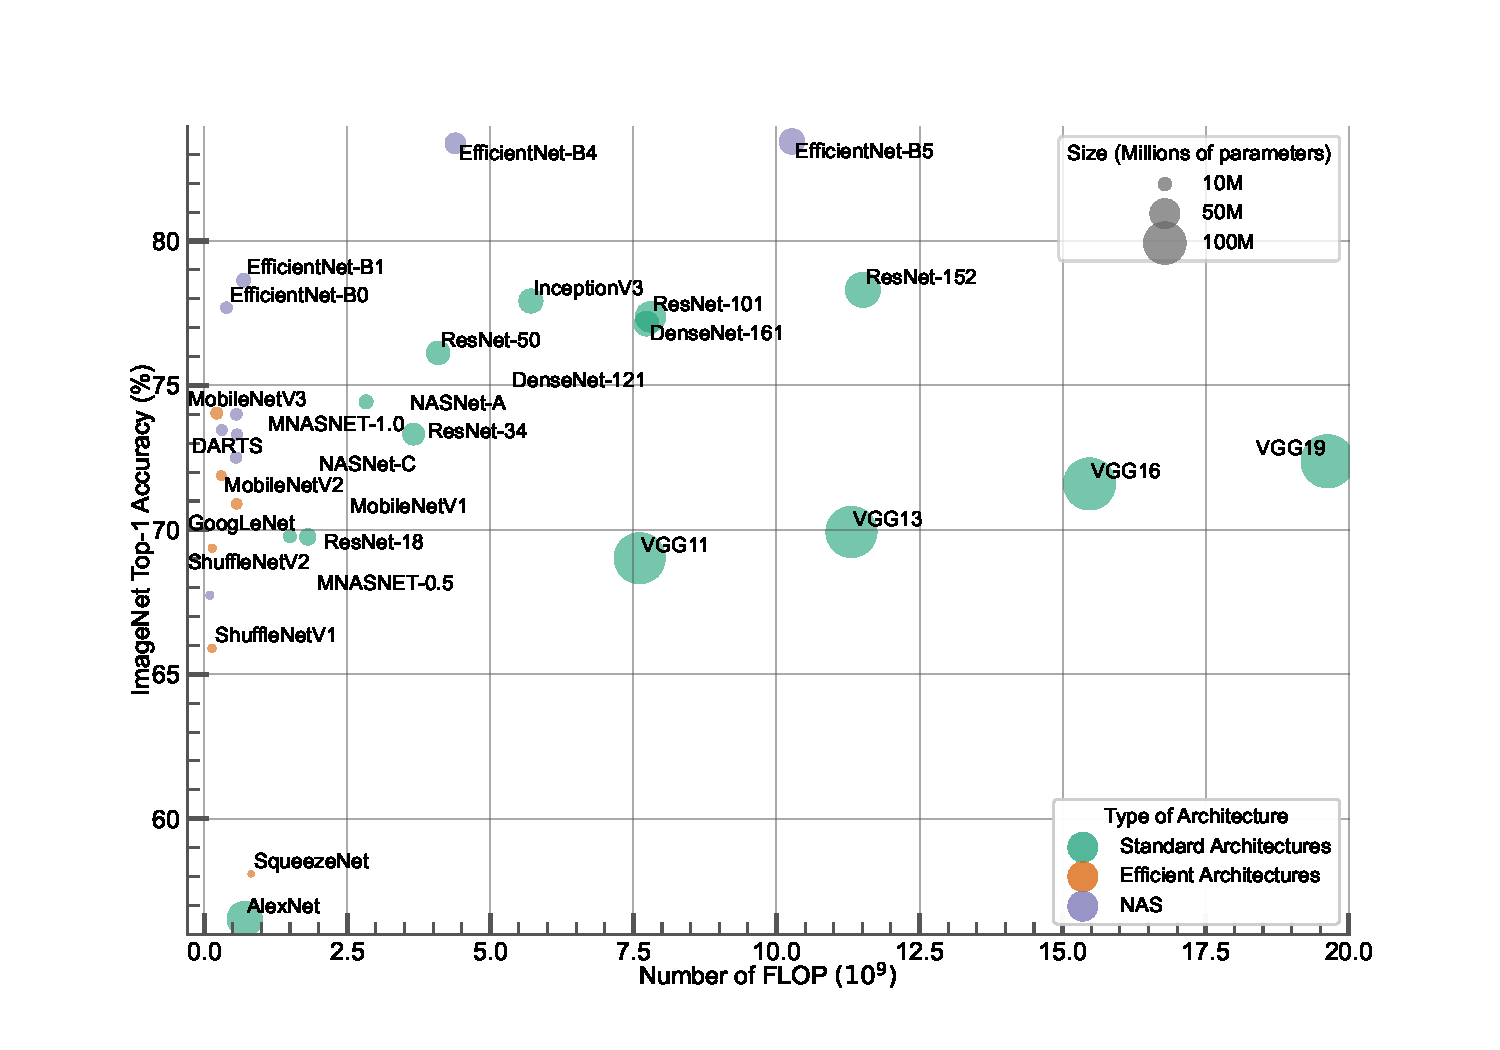
\includegraphics[width=0.70\textwidth]{chapter_sota/assets/network_sizes_normal_eff_nas.pdf}
  \caption{\Cref{fig:sota:net_sizes_std_eff} updated with the size and
    performance of architectures detailed in \cref{sec:sota:nas}. Best viewed in
    colours.}
  \label{fig:sota:net_sizes_std_eff_nas}
\end{figure}

\section{Compressing and Optimising an Existing Architecture}\label{sec:sota:refining_existing}

While the prior sections have primarily focused on constructing new, efficient
network architectures and mechanisms for automatic architecture discovery, this
part of the chapter transitions towards compressing and optimising existing neural
networks. The methods discussed in this section, namely \emph{quantisation},
\emph{binarisation} and \emph{pruning}, are specifically geared towards
leveraging and enhancing already existing architectures or trained models.
Instead of developing a new architecture, these techniques seek to make an
existing architecture more efficient by modifying its weights and connections.\\

\Cref{sec:sota:quantisation} delves into the methodologies of quantisation and
binarisation. These methods endeavour to reduce the numerical precision of
weights and activations in a network, without a significant drop in overall
performance. This process can significantly speed up computations and decrease
memory usage, contributing to the increased efficiency of a pre-existing
network, especially in environments with limited hardware or memory resources.\\

Subsequently, \cref{sec:sota:pruning} examines the application of
pruning techniques. Pruning refers to the elimination of redundant or
insignificant weights and connections in a network, leading to a sparser and
more effective architecture. Pruning an existing network can further enhance
efficiency by reducing the computational resources needed with a minimal or
controlled impact on the performance.\\

Through these methods, this section aims to demonstrate how the effectiveness of
existing neural networks can be optimised, thereby offering another viable path
towards generating more efficient models without creating new architectures from
scratch.\\

\subsection{Lower Precision Weights and Activations Representation}\label{sec:sota:quantisation}

Quantization is the process of converting continuous, high-resolution input
values into a lower-resolution and typically discrete representation.
Historically, the training of neural networks has largely relied on the use of
\ac{FP32}. \ac{FP32} has been the default choice due to its wide support across
various hardware platforms and software libraries, which has made it a practical
and convenient choice for the majority of machine learning tasks
\cite{sze2017efficient}. However, using \acl{FP32} is not always necessary, and
it is possible to constrain neural networks to use lower precision values,
effectively quantising its parameters or feature maps, while maintaining
compelling performances. Quantising a neural network can result in a reduced
memory footprint as well as faster computation if the operations are implemented
to leverage the specificity of the quantisation or paired with appropriate
hardware.\\

Quantising a neural network has been proposed as early as the 1990s
\cite{balzer1991weight,fiesler1990weight}. This later regains traction as
\citeauthor{37631} leveraged Single Input Multiple Data instructions (SIMD) of
x86 processor to speed up the fixed-point 8-bit operations \cite{37631}.
\citeauthor{gupta2015deep} \cite{gupta2015deep} used uniform quantisation with
fixed-point 16-bit representation and stochastic rounding to train neural
networks. Quantisation has also been applied together with K-means clustering
\cite{steinhaus1956division}. \cite{DBLP:journals/corr/HanMD15} uses K-means
clustering to iteratively compute a lookup table or \emph{code book} for the
weights. This codebook is later further compressed using Huffman coding
\cite{huffman1952method}. Note that this method is mostly useful for storage,
but for training or inference, the weights need to be decompressed and their
original value fetched in the code book before being used.\\

\noindent\textbf{Logarithmic quantisation.} Logarithmic quantisation provides
compelling alternatives to uniform quantisation. On the one hand, logarithmic
quantisation enables quantising weights with a larger dynamic range compared to
uniform or linear quantisation. On the other hand, multiplication can be
conveniently represented as an inexpensive bit shift operation if operands are
properly represented in the logarithmic base. This is particularly beneficial
for \ac{FPGA} implementations \cite{alemdar2017ternary}. To leverage this
potential speedup, \cite{DBLP:journals/corr/LinCMB15} forced the weight
representation to be a power of two and \cite{DBLP:conf/iclr/ZhouYGXC17}
improved this technique by applying it iteratively.\\

\begin{figure}[htbp]
  \centering
  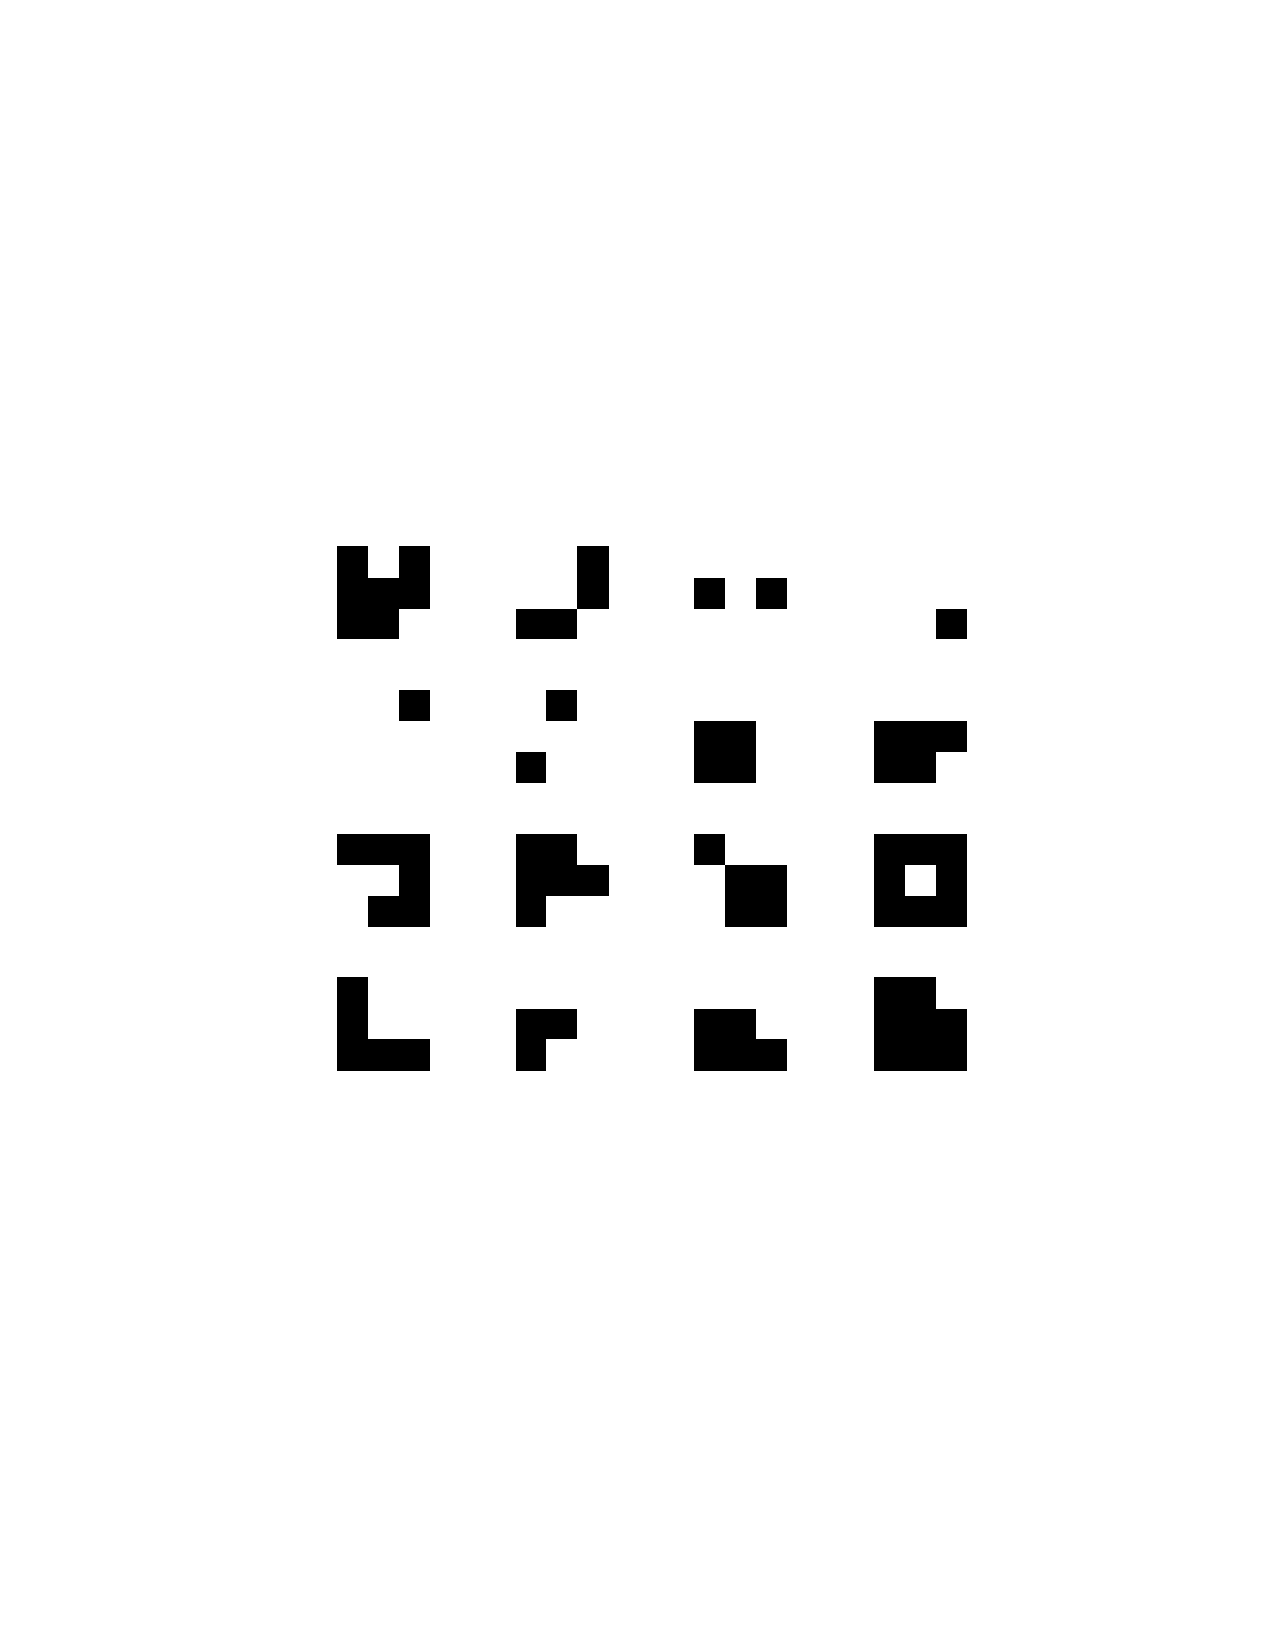
\includegraphics[width=0.40\textwidth,trim=5cm 9cm 5cm 9cm, clip]{chapter_sota/assets/binarised_kernels.pdf}
  \caption{Example of binarised kernels and activations in a convolutional
    layer. The kernels are taken from the first layer of a \ac{CNN} trained on CIFAR-10.
    Image taken from \cite{DBLP:conf/nips/HubaraCSEB16}.}
  \label{fig:sota:binarised_kernels}
\end{figure}

\noindent\textbf{Binarisation.} A more extreme version of the quantisation has
been proposed in \cite{courbariaux2015binaryconnect}, where the weight values
are either $-1$ or $+1$. The concept of minimising the bit-width of weights to a
bare minimum is called \emph{binarisation}. This allows for a dramatic
simplification of the computation in the neural network at the expense of a drop
in performance. Binarisation has been further developed in
\cite{DBLP:conf/nips/HubaraCSEB16}, where the authors proposed a method to
binarise both weights and activations (see examples of binarised kernels in
\cref{fig:sota:binarised_kernels}). DoReFa-Net \cite{zhou2016dorefa} built upon
the success of binarised neural networks and introduced the stochastic 8-bit
quantisation of the gradients during the backward pass to accelerate both
training and inference.\\

\noindent\textbf{When to quantise.} Quantisation methods that quantise weights
or activations after the training are called \ac{PTQ} methods. Quantising an
already existing network is a widely used technique in the most famous deep
learning framework \cite{ncnn,qnnpack,snapdragon,tensorrt}. Because they
quantise the weights after the training, \ac{PTQ} methods are fast and easy to
apply. However, they often introduce an irreversible information loss and a
performance drop that needs to be compensated for
\cite{DBLP:journals/ijon/LiangGWSZ21}. In order to solve this issue, several
works proposed to take into account the effect of quantisation on the weights
and feature maps during the training. These methods are called \ac{QAT} methods.
Such methods include BinaryConnect \cite{courbariaux2015binaryconnect}, which
use a variant of Bayesian inference called Expectation Back Propagation
\cite{DBLP:journals/corr/ChengSML15,DBLP:conf/nips/SoudryHM14}. Another
binarisation method uses \ac{STE} \cite{DBLP:journals/corr/BengioLC13} to bypass
the binarisation function in the backward pass
\cite{DBLP:conf/nips/HubaraCSEB16}. \ac{STE} is also employed for quantisation
in \cite{DBLP:conf/cvpr/JacobKCZTHAK18} which uses it together with \emph{fake
quantisation} nodes for 8-bit quantisation (see \cref{fig:sota:fake_quant}). The
fake quantisation nodes are injected inside the computation graph and simulate
the effect of quantisation in the forward pass.\\

Quantisation and binarisation are solutions to compress and accelerate neural
networks. The potential of these techniques is vast, as they offer significant
reductions in memory usage and enhanced computational speed when implemented
correctly and paired with suitable hardware. However, these benefits are not
without their drawbacks. On the downside, such techniques introduce a certain
degree of error which can result in a performance drop, especially if not
properly managed during the training process. This information loss is
particularly notable in the case of \acl{PTQ} methods, which necessitate
additional efforts to mitigate these performance impacts. To address this,
\ac{QAT} methods have been developed, which incorporate the effects of
quantisation during the training phase itself. The more extreme approach,
binarisation, further accentuates the advantages and disadvantages observed in
quantisation. While it offers extreme compression of neural networks, this often
comes at the cost of significant accuracy loss.\\


\begin{figure}[htbp]
  \centering
  \subfloat[Fake quantisation inference\label{fig:sota:fake_quant_inference}]{%
    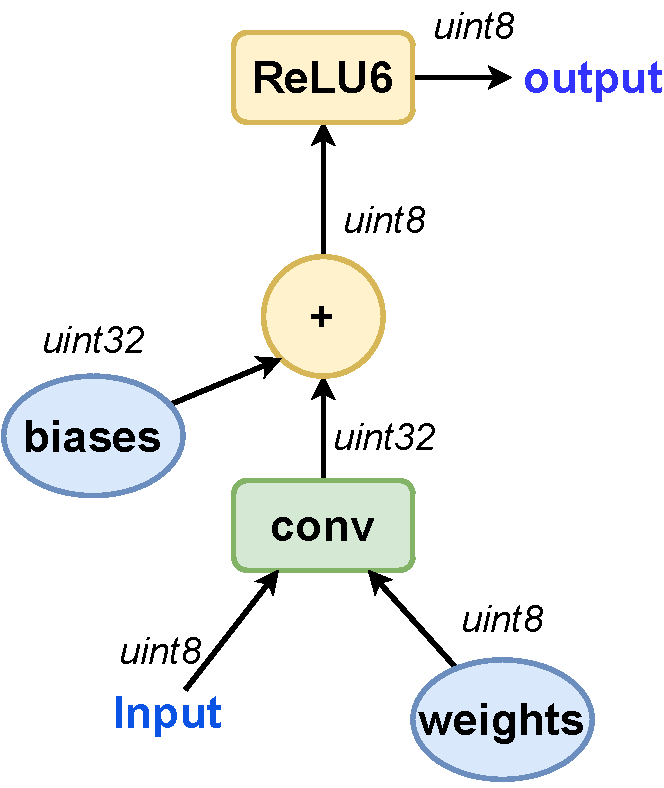
\includegraphics[height=6cm]{chapter_sota/assets/fake_quant_inference.pdf}}
  \subfloat[fake quantisation training\label{fig:sota:fake_quant_training}]{%
    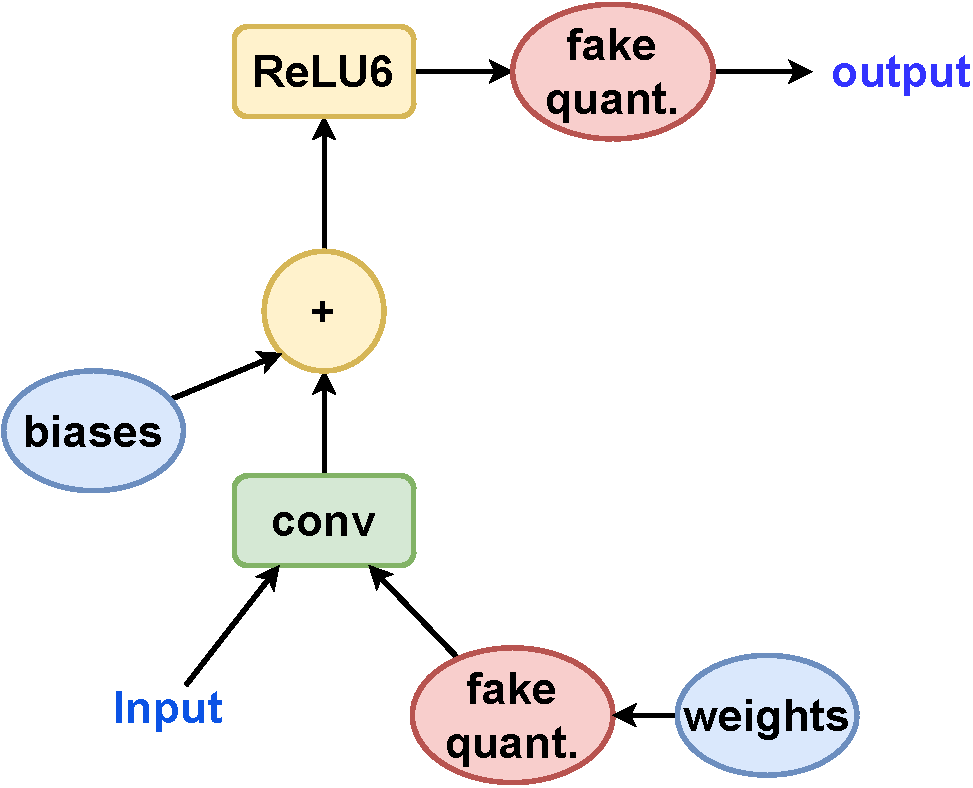
\includegraphics[height=6cm]{chapter_sota/assets/fake_quant_training.pdf}}
  \caption{Fake quantisation nodes (\emph{fake quant.}) are included in the
    computation graph of \cref{fig:sota:fake_quant_training}, whereas
    \cref{fig:sota:fake_quant_inference} represent the computaion graph used during
    inference. During the inference, weights are stored in \texttt{uint8} format,
    whereas the bias are not, because their computational overhead is
    negligible.\cite{DBLP:conf/cvpr/JacobKCZTHAK18}. Both illustrations are adapted
    from \cite{DBLP:conf/cvpr/JacobKCZTHAK18}.}
  \label{fig:sota:fake_quant}
\end{figure}

\subsection{Removing Weights and Connections}\label{sec:sota:pruning}

Lightweight neural networks can be obtained from a larger network through
pruning. Pruning is the process of removing weights or connections, identified
as redundant or unnecessary, while limiting to a minimum the impact on the
performance of the network. The identification of the latter, often referred to
as determining the \emph{saliency} of weights, has been a hot spot in the
pruning literature \cite{li2023model,cheng2017survey,liang2021pruning}. Pruning
a neural network removes weights and consequently reduces the theoretical
computational complexity of the network as well as its memory footprint.  The
fraction of weight removed during pruning is often denoted as the \emph{pruning
rate}, which is commonly defined as the fraction of the number of weights
removed from the original network over the number of initial weights in that
network. Arguably, the first pruning method, introduced in 1989, was based on
biased weight decay \cite{hanson1988comparing}. In the following years,
\citeauthor{DBLP:conf/nips/CunDS89} proposed a pruning method entitled Optimal
Brain Damage \cite{DBLP:conf/nips/CunDS89} that used the Taylor expansion of the
loss hessian matrix to identify the weights whose removal would have the least
impact on the loss. This method, and in particular the computation of the
hessian matrix were refined in Optimal Brain Surgeon
\cite{DBLP:conf/nips/HassibiS92,DBLP:conf/nips/HassibiSW93,DBLP:conf/icnn/HassibiSW93}.
As neural networks have become larger and more computationally intensive (see
\cref{sec:dlo:architectures,fig:dlo:net_sizes}), pruning has been receiving
increased attention as a method to compress the latter. Pruning methods can be
classified into two categories: \emph{structured} and \emph{unstructured}.\\


\begin{figure}
  \centering
  \subfloat[Structured pruning\label{fig:sota:structured_pruning}]{%
    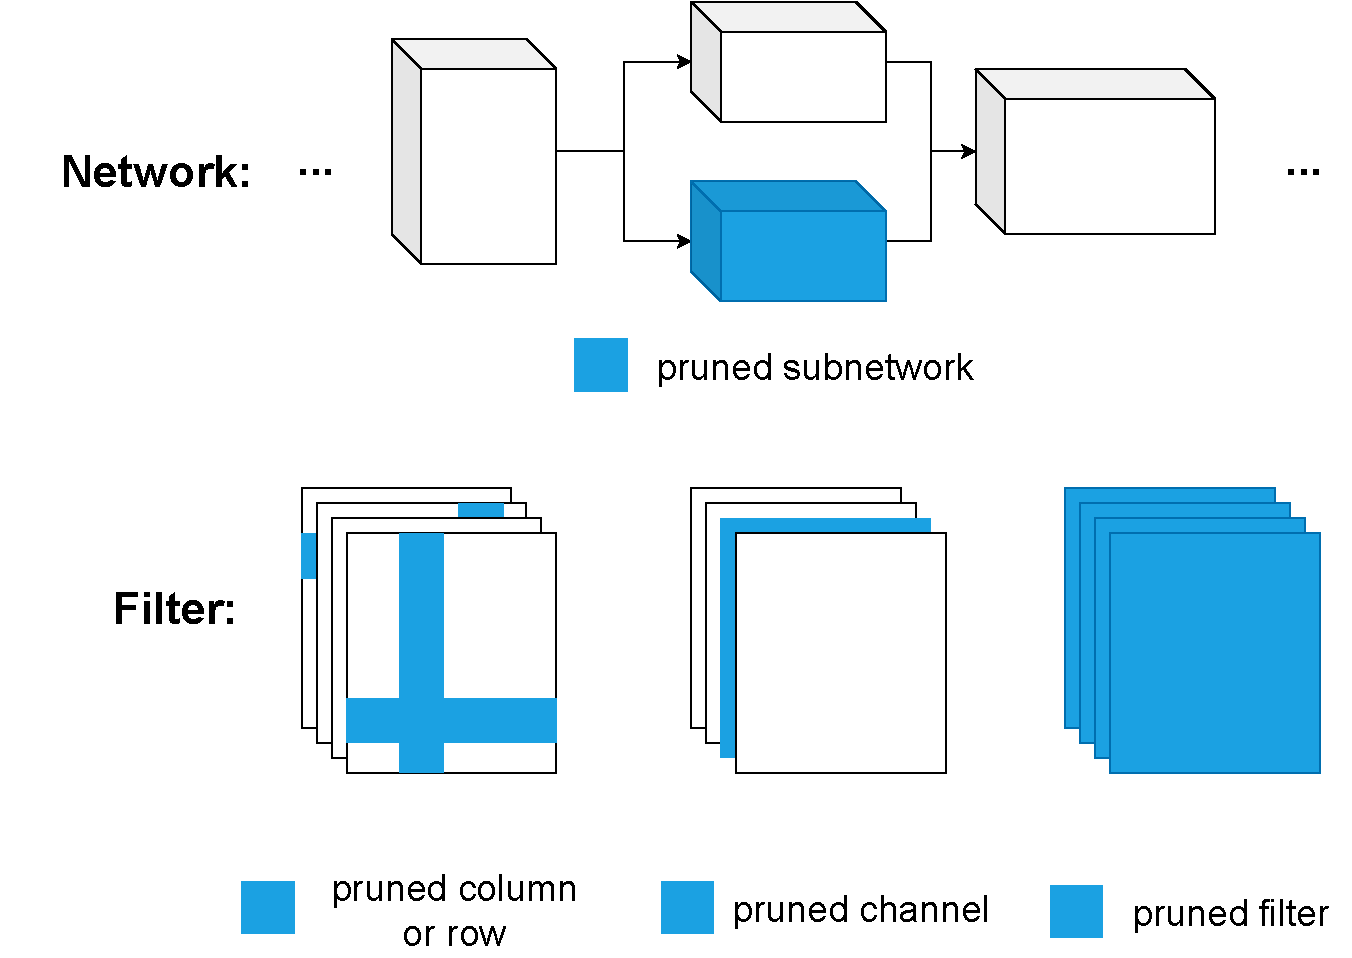
\includegraphics[width=0.6\textwidth]{chapter_sota/assets/structured_pruning.pdf}}
  \hspace{0.09\textwidth}
  \subfloat[Unstructured pruning\label{fig:sota:unstructured_pruning}]{%
    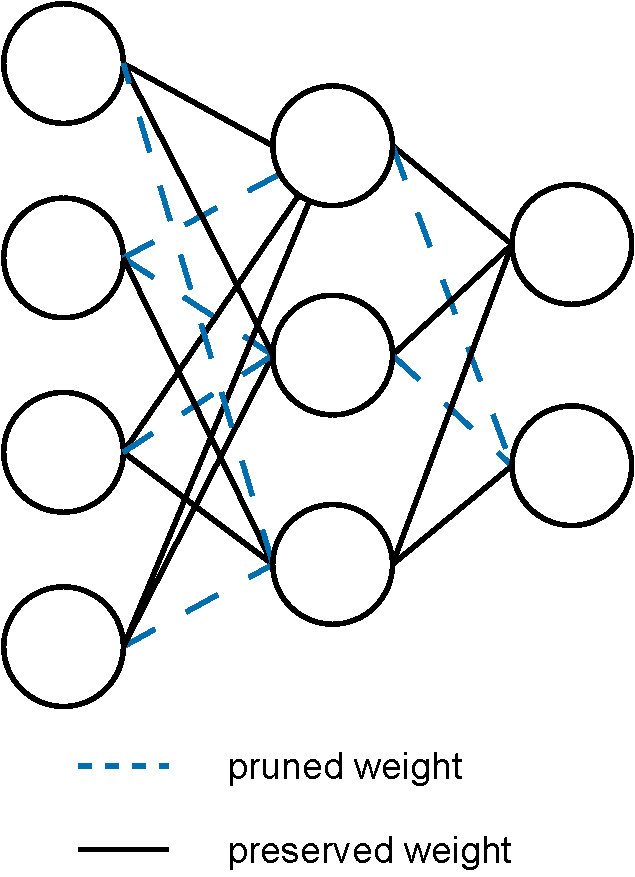
\includegraphics[width=0.3\textwidth]{chapter_sota/assets/unstructured_pruning.pdf}}
  \caption{Conceptual illustrations of structured and unstructured pruning.}
  \label{fig:sota:pruning}
\end{figure}

\noindent\textbf{Structured pruning.} Structured pruning involves the removal of
entire structural components of the network, such as rows, columns, channels,
filters, layers or even whole subnetworks (note that pruning a channel in layer
$\ell+1$ implies pruning a filter in layer $\ell$, and vice-versa). This type of
pruning results in regular\footnote{regular in this context means that all
weight tensors are dense and that the acceleration of computations does not rely
on sparse computing enhancement.} network structures that are easier to exploit
on typical hardware and do not necessitate a specific sparse computing library
or hardware, making it an attractive approach for practical deployment. To some
extent, structured pruning can be seen as a subcategory of \acl{NAS}
(\cref{sec:sota:nas}), where the search space would be the structure of the
network to be pruned. Structured pruning leads to reduced computation complexity
as well as significant memory footprint reduction, however, it also presents
unique challenges. The impact of removing structural components can be much
greater than eliminating individual weights, hence, structured pruning often
requires more careful consideration of the trade-off between the model
performance and complexity reduction. Since structured pruning operates on a
coarser scale, it typically results in lower pruning rates compared to
unstructured pruning.\\


\noindent\textbf{Weight-dependant structured pruning.} One of the main
categories of structured pruning for \ac{CNN} is weight-dependent pruning. This
strategy assesses the importance of filters based on their respective weights.
The Pruning Filter for Efficient ConvNets method
\cite{DBLP:conf/iclr/0022KDSG17} focuses on the filter norms as their saliency
indicator. Filters with smaller $\ell_1$ norms, which result in weak
activations, are assumed to contribute less to the final classification
decision, hence they become the prime candidates for pruning.  The Filter
Pruning via Geometric Median method \cite{DBLP:conf/cvpr/HeLWHY19} calculates
the geometric median of a set of filters and prunes those filters that are
nearest to this geometric median, rather than the ones considered less important
by \cite{DBLP:conf/iclr/0022KDSG17}. The filters close to the geometric median
are considered by \citeauthor{DBLP:conf/cvpr/HeLWHY19} to be redundant with
other filters in the same layers. \citeauthor{DBLP:conf/cvpr/WangLW21} used
another approach to determine redundancy in \cite{DBLP:conf/cvpr/WangLW21}: The
filters are organized into a graph based on their proximity in the space in
which they are defined. A redundancy metric is computed for each graph and the
least important filters are pruned in the graph with the highest redundancy (as
per the authors, any other method for filter importance evaluation can be used
\cite{DBLP:conf/iclr/0022KDSG17,DBLP:journals/access/PolyakW15,DBLP:conf/iclr/MolchanovTKAK17}).
This process is iteratively applied until the targeted pruning rate is reached.
These weight-dependent strategies tend to be straightforward and usually demand
lower computational costs compared to other methods
\cite{DBLP:journals/corr/abs-2303-00566}. They provide an intuitive
understanding of how different filters contribute to the overall network
performance based on their weight characteristics. \\


\begin{figure}[htbp]
  \centering
  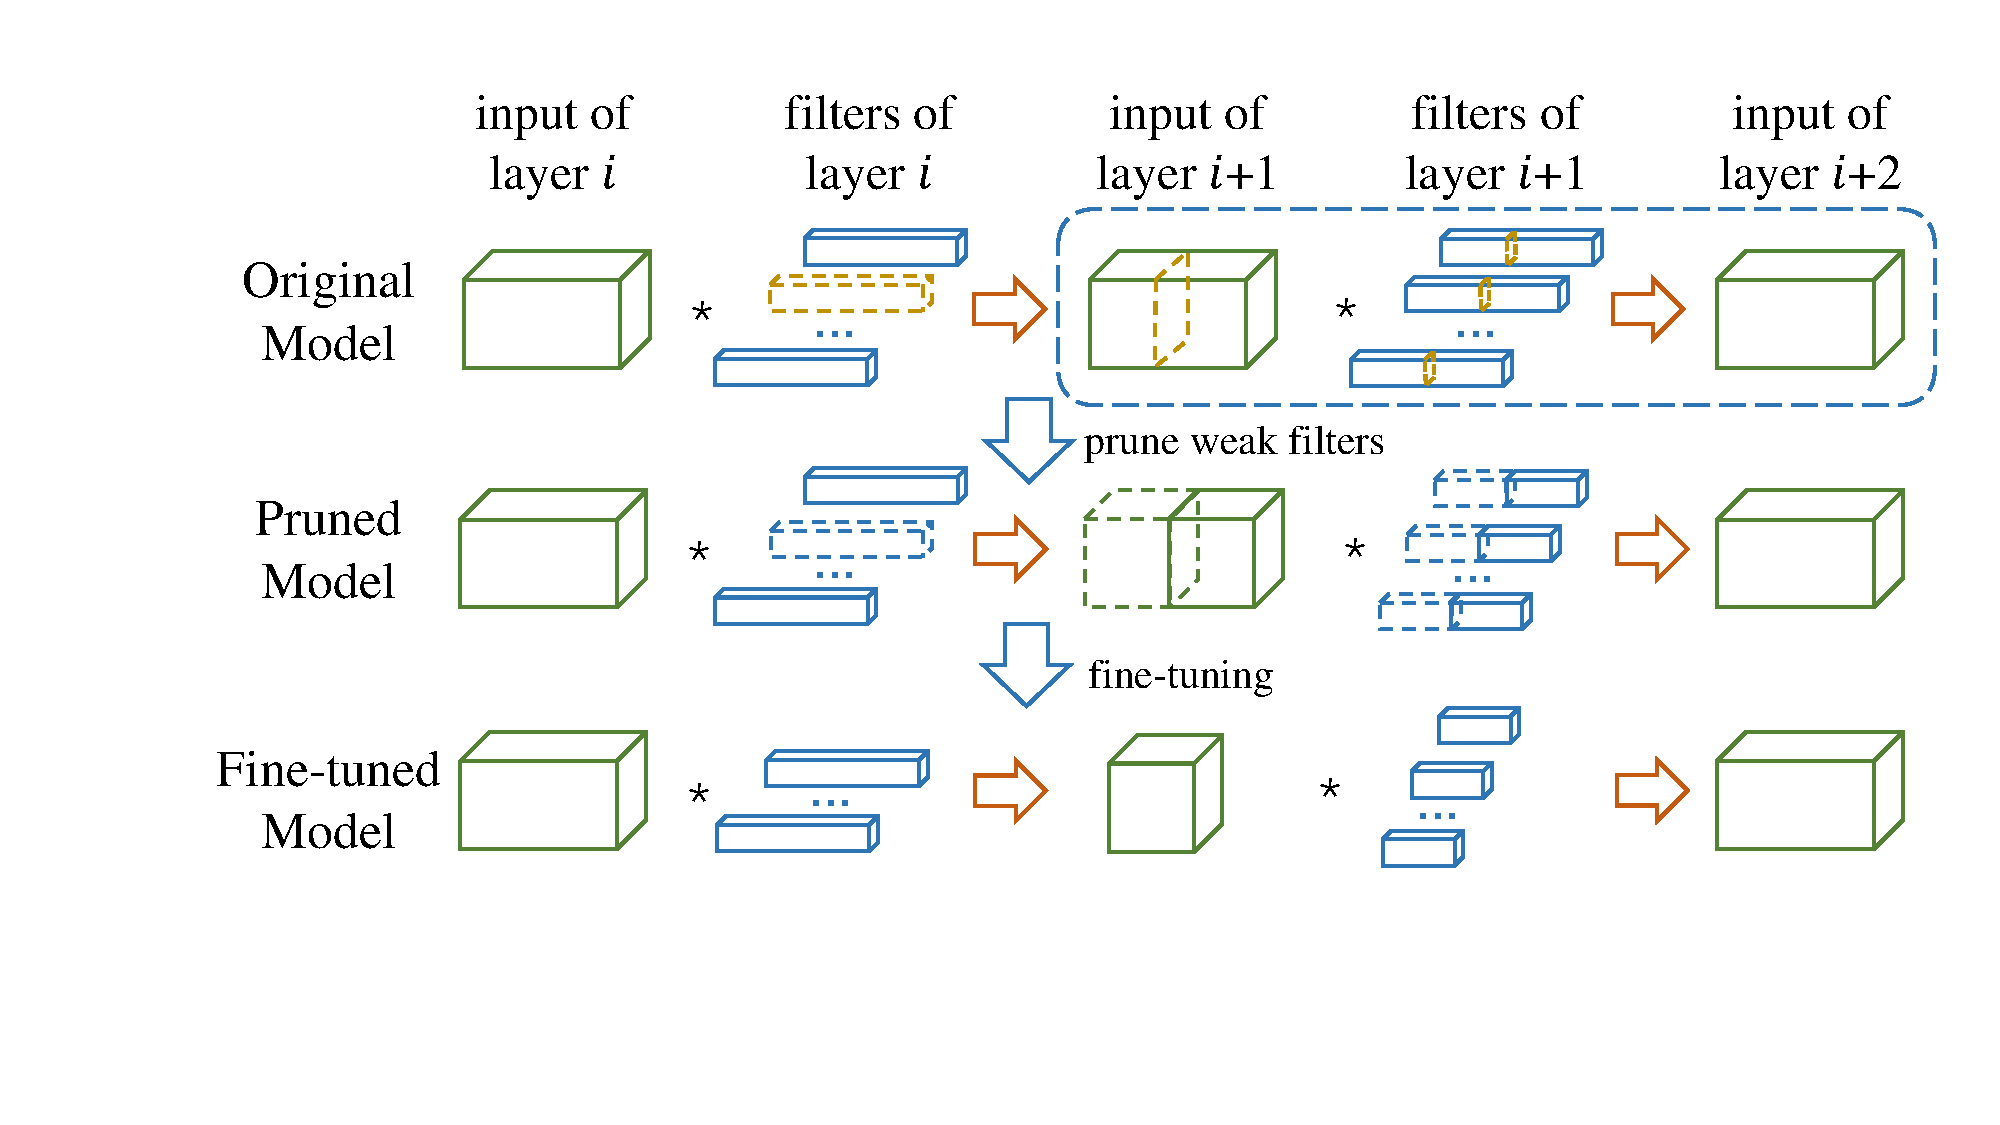
\includegraphics[width=0.8\textwidth]{chapter_sota/assets/thinet.pdf}
  \caption{Illustration Scheme of ThiNet. The dotter filters and corresponding
    channels are the ones to be pruned. Once they are removed, the pruned network
    is fine-tuned. Image taken from \cite{DBLP:conf/iccv/LuoWL17}}
  \label{fig:sota:thinet}
\end{figure}

\noindent\textbf{Activation-based structured pruning.} Another prominent
category of structured pruning is activation-based pruning, where
\emph{activation} denotes the result yielded by a layer for given input data.
This method takes advantage of activation maps (also called feature maps) for
filter pruning. Removing a channel in a feature map is equivalent to removing
the filter that computed this channel. \citeauthor{DBLP:conf/iccv/HeZS17}
proposed a method to prune filters based on a LASSO regression selection while
minimising the least square reconstruction error or the feature map
\cite{DBLP:conf/iccv/HeZS17}. \citeauthor{DBLP:journals/corr/HuPTT16}
capitalised on the abundance of zeros in feature maps that follow the \ac{ReLU}
activation function. They introduced the method called Average Percentage of
Zeros (APoZ) that identifies channels in the feature map with a high count of
null outputs. These channels, which contribute minimally to the final outcome,
can hence be pruned. While the aforementioned methods consider only the feature
map of the layer to be pruned, techniques like ThiNet
\cite{DBLP:conf/iccv/LuoWL17} and Approximated Oracle Filter Pruning
\cite{DBLP:conf/icml/DingDGHY19} exploit the relationships between layers to
guide pruning. They take into consideration the effect a filter removal in one
layer has on the next, allowing for more contextual pruning decisions. More
globally, approaches such as Neuron Importance Score Propagation
\cite{DBLP:conf/cvpr/Yu00LMHGLD18} and Discrimination-aware Channel Pruning
\cite{DBLP:conf/nips/ZhuangTZLGWHZ18} consider the holistic effect of removing a
filter. They aim to understand and quantify the total impact on network
performance when a specific filter is removed, accounting for cascading effects
across all layers.\\

\noindent \textbf{Regularisation-based structured pruning.} Other methods learn
structured sparse networks by introducing various sparsity regularizers. Some
methods focus on \acl{BN} parameters, employing methods like Gated Batch
Normalisation \cite{DBLP:conf/nips/YouYYM019} and Network Slimming
\cite{DBLP:conf/iccv/LiuLSHYZ17}. These methods aim to push certain BN
parameters towards zero, effectively disabling corresponding channels and
inducing sparsity. Network Slimming applies a $\ell_1$ regularisation on the
scaling factors $\gamma$ of the \ac{BN} \cite{DBLP:conf/iccv/LiuLSHYZ17},
whereas \cite{DBLP:conf/nips/YouYYM019} adds the $\ell_1$ regularisation on
scalar factors associated with feature map channels.
\citeauthor{DBLP:conf/icml/KangH20} use \ac{BN} parameters to craft a mask that
prunes channels whose output is likely to be null once evaluated by the
\ac{ReLU} \cite{DBLP:conf/icml/KangH20}. \\

\begin{figure}[htbp]
  \centering
  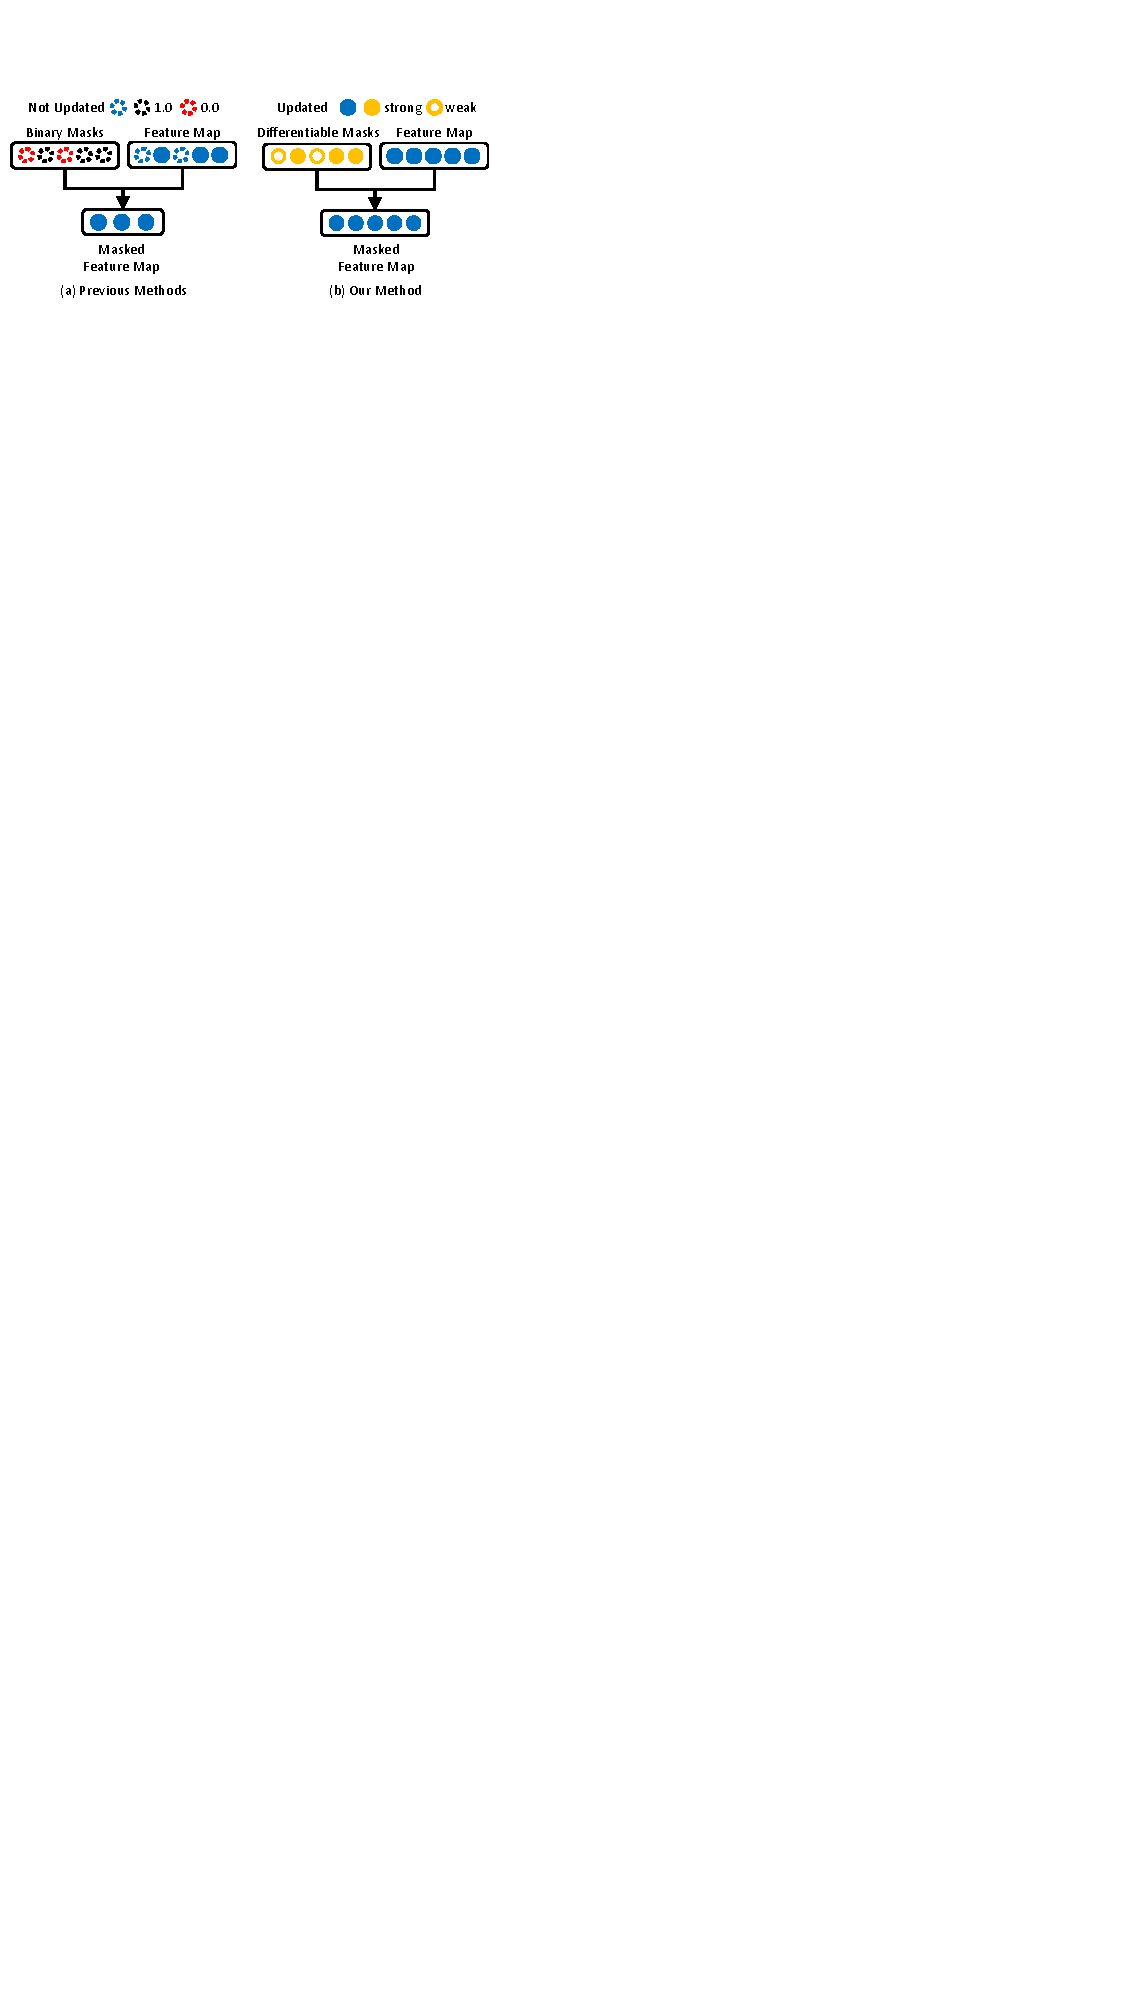
\includegraphics[width=0.8\textwidth,trim=0 0.4cm 0 0, clip]{chapter_sota/assets/operation_aware.pdf}
  \caption{Comparison of the method described in \cite{DBLP:conf/icml/KangH20}
    (right) and standard channel pruning (left). The differentiable mask allows
    for a soft pruning that can be reverted during the training. Image taken
    from \cite{DBLP:conf/icml/KangH20}}
  \label{fig:sota:operation_aware}
\end{figure}


\noindent \textbf{Taylor Expansion-based structured pruning.} The Taylor
Expansion is a tool that can be used to approximate the change in the loss
function due to pruning. Early unstructured pruning methods, Optimal Brain
Damage \cite{DBLP:conf/nips/CunDS89} and Optimal Brain Surgeon
\cite{DBLP:conf/icnn/HassibiSW93} used Taylor expansion of the hessian matrix to
remove weights with the least impact on the loss function. More recently, in
\cite{DBLP:conf/iclr/MolchanovTKAK17},
\citeauthor{DBLP:conf/iclr/MolchanovTKAK17} used first-order Taylor expansion of
the loss function to compute the importance score and prune the feature maps.
This was later refined in \cite{DBLP:conf/cvpr/MolchanovMTFK19} where the
authors computed the importance score on the weight, rather than the feature
maps, to lower memory consumption.\\

\noindent\textbf{Variational structured pruning.} Variational Bayesian methods
provide a way to tackle the computationally intensive process of inferring
posterior probability distributions in large data sets, by approximating the
posterior distribution with a variational distribution \cite{fox2012tutorial}.
Specific methods like Variational Pruning \cite{DBLP:conf/cvpr/ZhaoNZZZT19} and
Recursive Bayesian Pruning \cite{DBLP:conf/iccv/Zhou0W019} use this approach to
create more effective and stable pruning mechanisms for neural networks.
Variational Pruning, models channel importance as random variables, utilizing
the centrality property of the Gaussian distribution to induce sparsity
\cite{DBLP:conf/cvpr/ZhaoNZZZT19}, while \cite{DBLP:conf/iccv/Zhou0W019} targets
the posterior of redundancy, assuming inter-layer dependency among channels.\\


\noindent\textbf{Dynamic structured pruning.} Dynamic pruning represents a
different approach in which neural networks are pruned during both training and
inference, which facilitates maintaining the model representation capability and
offers superior resource consumption-accuracy trade-offs. In the training phase,
Dynamic Network Surgery \cite{DBLP:conf/nips/GuoYC16} introduces the concept of
dynamic pruning through an unstructured approach. This method applies a binary
mask indicating the importance of weights and updates it alternately with all
the weights, allowing incorrectly pruned parameters an opportunity to revive.
Soft Filter Pruning \cite{DBLP:conf/ijcai/HeKDFY18} implements a structured
version of dynamic pruning. Instead of employing a fixed mask throughout the
training, which could limit the optimization space, Soft Filter Pruning
dynamically generates masks based on the $\ell_2$ norm of filters at every
epoch. The dynamic nature of Soft Filter Pruning allows soft-pruned filters to
be updated in the next epoch, with new masks being formed based on the updated
weights. Focusing on the inference stage, \citeauthor{DBLP:conf/nips/LinRLZ17}
introduced Runtime Neural Pruning \cite{DBLP:conf/nips/LinRLZ17} which employs a
unique framework consisting of a \ac{CNN} backbone and a recurrent neural
network as a decision network. This approach enables the model to adapt to the
properties of different input images by dynamically adjusting its complexity.
For easier tasks or simpler images, the network can become sparser, saving
computational resources. Deep Reinforcement Learning pruning
\cite{DBLP:conf/nips/ChenCP20} learns both the static and dynamic importance of
channels. The static importance refers to the channel's relevance for the entire
dataset, while the dynamic importance is tied to a specific input. Deep
Reinforcement Learning pruning \cite{DBLP:conf/nips/ChenCP20} applies
reinforcement learning to generate a unified pruning decision based on these two
aspects of channel importance. More recently,
\citeauthor{DBLP:conf/cvpr/ElkerdawyE0R22} recently introduced Fire Together
Wire Together \cite{DBLP:conf/cvpr/ElkerdawyE0R22}, another dynamic pruning
method that treats pruning as a self-supervised binary classification problem.
It employs a prediction head to train learnable binary masks and uses a crafted
ground truth mask to guide the learning after each convolutional layer. This
head takes advantage of the \ac{ReLU} activation function, which zeros out
negative values, to identify the filters that will yield zero activations based
on the input and that will be subsequently pruned.\\

As previously discussed, structured pruning removes indivisible groups of
weights and therefore yields regular network architectures that can be
implemented in standard deep learning frameworks in a straightforward way.
Despite its practicality, structured pruning enforces a strong topological prior
by pruning entire groups of weights from the original network, which
consequently leads to a lower sparsity rate compared to its counterpart,
unstructured pruning. Unstructured pruning provides a more flexible approach by
removing individual weights from the original network structure. This process
not only offers greater adaptability compared to structured pruning, but also
results in higher pruning rates.\\

\noindent\textbf{Unstructured pruning.} In the early stages, unstructured
pruning methodologies identified weights that could be eliminated based on their
influence on the Hessian of the loss function
\cite{DBLP:conf/nips/CunDS89,DBLP:conf/icnn/HassibiSW93,DBLP:conf/nips/HassibiSW93}.
A simpler and more tractable strategy for larger networks was later introduced
by \citeauthor{DBLP:conf/nips/HanPTD15} in \cite{DBLP:conf/nips/HanPTD15},
suggesting a straightforward heuristic: the pruning of weights with the smallest
magnitude (\emph{i.e.} absolute value), also referred to as \emph{magnitude
pruning}. This technique presented in \cite{DBLP:conf/nips/HanPTD15} devises an
iterative method wherein a portion of the smallest magnitude weights are
removed, followed by the retraining of the network to compensate for the drop of
the accuracy. This cycle is reiterated until the preferred level of sparsity is
attained. Furthermore, magnitude pruning has been used together with
quantisation and compression techniques to minimise the storage footprint of a
network \cite{DBLP:journals/corr/HanMD15}. Magnitude pruning has also been used
in energy-efficient \ac{CNN} design, as detailed in
\cite{DBLP:conf/cvpr/YangCS17}. In this research, the energy consumption of each
layer is evaluated, and the layers with the highest energy expenditure are
pruned using unstructured magnitude pruning. This layer is then fine-tuned to
retain the network accuracy. This process is repeated iteratively until a
noticeable drop in accuracy is observed. Dynamic Network Surgery
\cite{DBLP:conf/nips/GuoYC16} puts forward a derivative of magnitude pruning. A
mask, whose value is updated during training, is computed for each weight. This
mask is used to stochastically prune a weight or splice\footnote{to splice is
the verb used by the authors (\citeauthor{DBLP:conf/nips/GuoYC16}) to denote the
reactivation of a weight that was previously pruned} it. The saliency of the
weights is ascertained based on the magnitude of the associated mask.\\

\noindent\textbf{Effective subnetworks.} More recently, unstructured pruning
researches focus on the discovery of small sub-networks inside the original
network. In other words, to identify a subset of weight that can perform, under
certain conditions or assumptions, as well as the original network. Most
notably, the Lottery Ticket Hypothesis \cite{DBLP:conf/iclr/FrankleC19} states
that within a large, randomly initialized neural network, there exist
sub-networks or \emph{Lottery Tickets} that are capable of training effectively
when isolated from the rest of the weights. These smaller networks, found by
pruning the smallest magnitude weights from the trained original network, are
observed to train faster and achieve comparable or even superior performance
with respect to the original network. The \emph{lottery ticket} is found by
training the original network up to convergence, then pruned with magnitude
pruning and finally, the remaining weights are reinitialized to their original
values, it is to say the value they had before the training even started. The
resulting sub-network is the \emph{lottery ticket}. This research sparked
significant interest and various works: \cite{DBLP:conf/nips/ZhouLLY19} proposed
an analysis of the results presented in \cite{DBLP:conf/iclr/FrankleC19}. These
results \cite{DBLP:conf/iclr/FrankleC19} have been extended to larger networks
in \cite{DBLP:journals/corr/abs-1903-01611}, the necessity of training the
original network to convergence to find the Lottery Tickets has been challenged
in \cite{DBLP:conf/iclr/LiuSZHD19}. The existence of the \emph{lottery ticket}
(or in other words the subnetwork) has been theoretically proven in
\cite{DBLP:conf/icml/MalachYSS20} and the requirements on the theoretical size
of the original network have been later refined in
\cite{DBLP:conf/nips/PensiaRNVP20,DBLP:conf/nips/OrseauHR20}.\\

\section{Positioning}

Within the various deep neural network compression methods presented in this
chapter, we choose to focus specifically on pruning in the context of supervised
image classification. Among various types of pruning, our interest goes towards
structured pruning due to the flexibility it offers, in particular, its
potential for achieving high pruning rates compared to unstructured pruning.\\

\noindent Our decision to work on pruning is rooted in the following
considerations:
\begin{itemize}
  \item First, pruning allows the creation of lightweight networks while
  preserving or sometimes improving the performance of the original network.

  \item Then, pruning integrates well with other compression techniques and can
  be applied in conjunction with them, on any kind of architecture.

  \item  Finally, pruning does not necessitate the creation and development of
  an architecture from scratch. It can be applied to an already existing
  architecture to compress it, which makes it possible to develop small,
  lightweight networks without the need for extensive research into the creation
  of the base architecture. This approach allows freeing exploration and
  research and development efforts that can be allocated to other topics.

\end{itemize}

Despite its numerous advantages, pruning is not without challenges. One such
challenge is the identification of the weights to be preserved. This is a topic
that is the subject of many works detailed in this chapter. Additionally, the
preserved weights typically require fine-tuning, which can impose a substantial
computational cost. This process of fine-tuning can be both time-consuming and
resource-intensive.\\

\Cref{chap:chapter1} delves into the fine-tuning issue and presents a new
pruning method that circumvents the need for the expensive fine-tuning step. Its
budget loss together with the weight reparametrisation allows for joint
optimisation of the topology and the weights of the network without the need for
auxiliary variables. As a result, the obtained lightweight networks preserve
accuracy after effective pruning and do not require fine-tuning. Furthermore,
\cref{chap:chapter2} tackles the challenge of identifying relevant weights
without even having to train them. It proposes a method of topology selection
given a set of untrained weights that achieves compelling performances, thereby
also sidestepping the fine-tuning. In contrast to other methods, the optimal
pruning rate is discovered in one shot by our pruning strategy that circumvents
the costly gird search for its value. This innovative approach opens up new
possibilities for further reducing the computational costs associated with
pruning and provides a new direction for future research in this area, as well
as neural network training without weight tuning in general.\\


\section{Conclusion}


The evolution of neural networks, along with the growing demand for their
deployment in resource-constrained environments, has underlined the need for
neural network compression techniques. This chapter has examined the
state-of-the-art methodologies for reducing the computational demands and memory
footprints of deep neural networks, thereby facilitating their usage in a
variety of application domains.\\

First, we explored \cref{chap:dlo} the historical progression and the major
architectures of deep neural networks, illustrating the connection between their
complexity and performance. Then, in this chapter, we first investigated the
techniques for accelerating computations within neural networks, emphasising the
role of fast convolution techniques in reducing both runtime and computational
resources. Our focus then shifted to \acl{KD}, a paradigm that allows the
transfer of knowledge from a large, complex network to a smaller, more efficient
one. The core idea is to teach a lightweight student network to mimic the
behaviour of a teacher network, thus achieving comparable performance with a
reduced footprint. Next, we delved into efficient architecture design methods,
including bespoke architectures designed to minimise size while maintaining
performance, and \acl{NAS} strategies for automating the discovery of optimal
architectures. Lastly, we addressed the strategies for compressing and
optimising existing neural networks, considering both quantisation and
binarisation techniques that lower the numerical precision of weights and
activations, as well as pruning techniques that remove redundant or
insignificant weights and connections, resulting in sparser and more
computationally efficient models. In conclusion, these techniques provide a
multi-faceted approach to neural network compression and acceleration, with each
offering unique advantages and trade-offs.\\

The next chapters will present approaches to neural network compression based on
pruning. The \cref{chap:chapter1} details our first contributions that consist
in a method to simultaneously train and prune neural networks while matching a
budget. This method allows bypassing the need for the finetuning step present in
most methods based on magnitude pruning by jointly optimising the topology and
the weights without the need for additional auxiliary parameters. 